


\thispagestyle{empty}
\mbox{}
\vfill
\begin{center}
    \textit{This page is left intentionally blank.}
\end{center}
\vfill
\newpage
\noindent


\begin{multicols}{2}

\noindent
---\textbf{System} (\ref{sec:high})---\textbf{Threads:} Hardware threads (CPU cores) each
may run one software thread (program) at a time. Switching,
between threads is context switching (overhead). E.g.,
Go manages internal thread pools, offering it to the OS,
reducing overhead.
\textbf{Thread Comm:} Inter-process communication (IPC), 
threads communicate via shared memory (e.g., channels, pipes, virtual memory).
\textbf{Conc. \& Parrelism:} Concurrency shuffles tasks,
parallelism runs tasks simultaneously (threads).
\textbf{Dist. Conn:} A client connects to a server (client-server model), a TCP conn. (FIFO)
secures the line, the RPC (remote procedure call) abstracts
dist. communication.
\textbf{Races \& Deadlocks:} Data race, two threads manipulating shared data (reads-onlys are fine).
\textbf{Mutexes:} Placing locks around shared data, stopping concurrent access.
\textbf{RPC Fail Models:} At-least-once, client retries until a response is received.
Rads are fine, writes cause race conditions. At-most-once, server handles dupes, clients
send unique IDs (cached responses). Exactly-once, both at-least-once and at-most-once.
\textbf{(a)sync:} Asynchronous, non-blocking, no waiting for a response. Synchronous, blocking, waiting for a response.
\textbf{(un)buffered-channers:} Unbuffered, sender waits for receiver on some thread to receive message. Buffered, sender sends message(s) to a buffer, takes one at a time.
\textbf{Task, Data, Pipeline Parallelism:} Task, same data, different tasks. Data, same task, different data. Pipeline, task split into dependent stages, independent stages run in parallel.
\textbf{Time Accr:} Physical clocks drift due to hardware limitations. Atomic clocks, have insignificant drift. NTP (network time protocol), 
utilizes GPS satellites to sync time, to a ground truth clocks, which propagates time to other systems.---\textbf{Logical Time} (\ref{sec:logical_clocks})---\textbf{Lamport Clocks:} 
Lamport Clocks, $(t_p, p)$, $t_p$ time of process $p$, monotonically increases for each event/send (Total Ordering). 
Receivers $q$ resolve time differences, $t_q = max((t_p+1), t_q)$ (send vs. local time). Given 
two events $a$ \& $b$, timestamps $t(a)$ \& $t(b)$, with $r$ trace: $a\to_r b \implies t(a) < t(b)$ (causal ordering);
$t(a) \geq t(b) \implies a \not\to_r b$ (concurrent); $(t(a) = t(b) \land a\gg b) \implies a \to_r b$, s.t., ($\gg$) rep. process order.
\textbf{Non-causal:} $(a\ll b):= (a \not\to_r b) \land (b\not\to_r a)$ (concurrent).
\textbf{Vector Clocks:} Operate as an array of Lamport clocks, index is process $p_i$, and value is $t_{p_i}$ (time); However, sends do not increment $t_{p_i}$.
Given timestamps $a$ \& $b$, if all indexes in $a$ are larger than $b$, $a\to_r b$. If some in $a$ are larger than $b$, vice versa, $a<>b$ (non-comparable, concurrent, partial ordering).

\noindent
TaskPar. DataPar. PipePar. La\&Ve.Clock:
\noindent
\rule{\linewidth}{0.4pt}\\
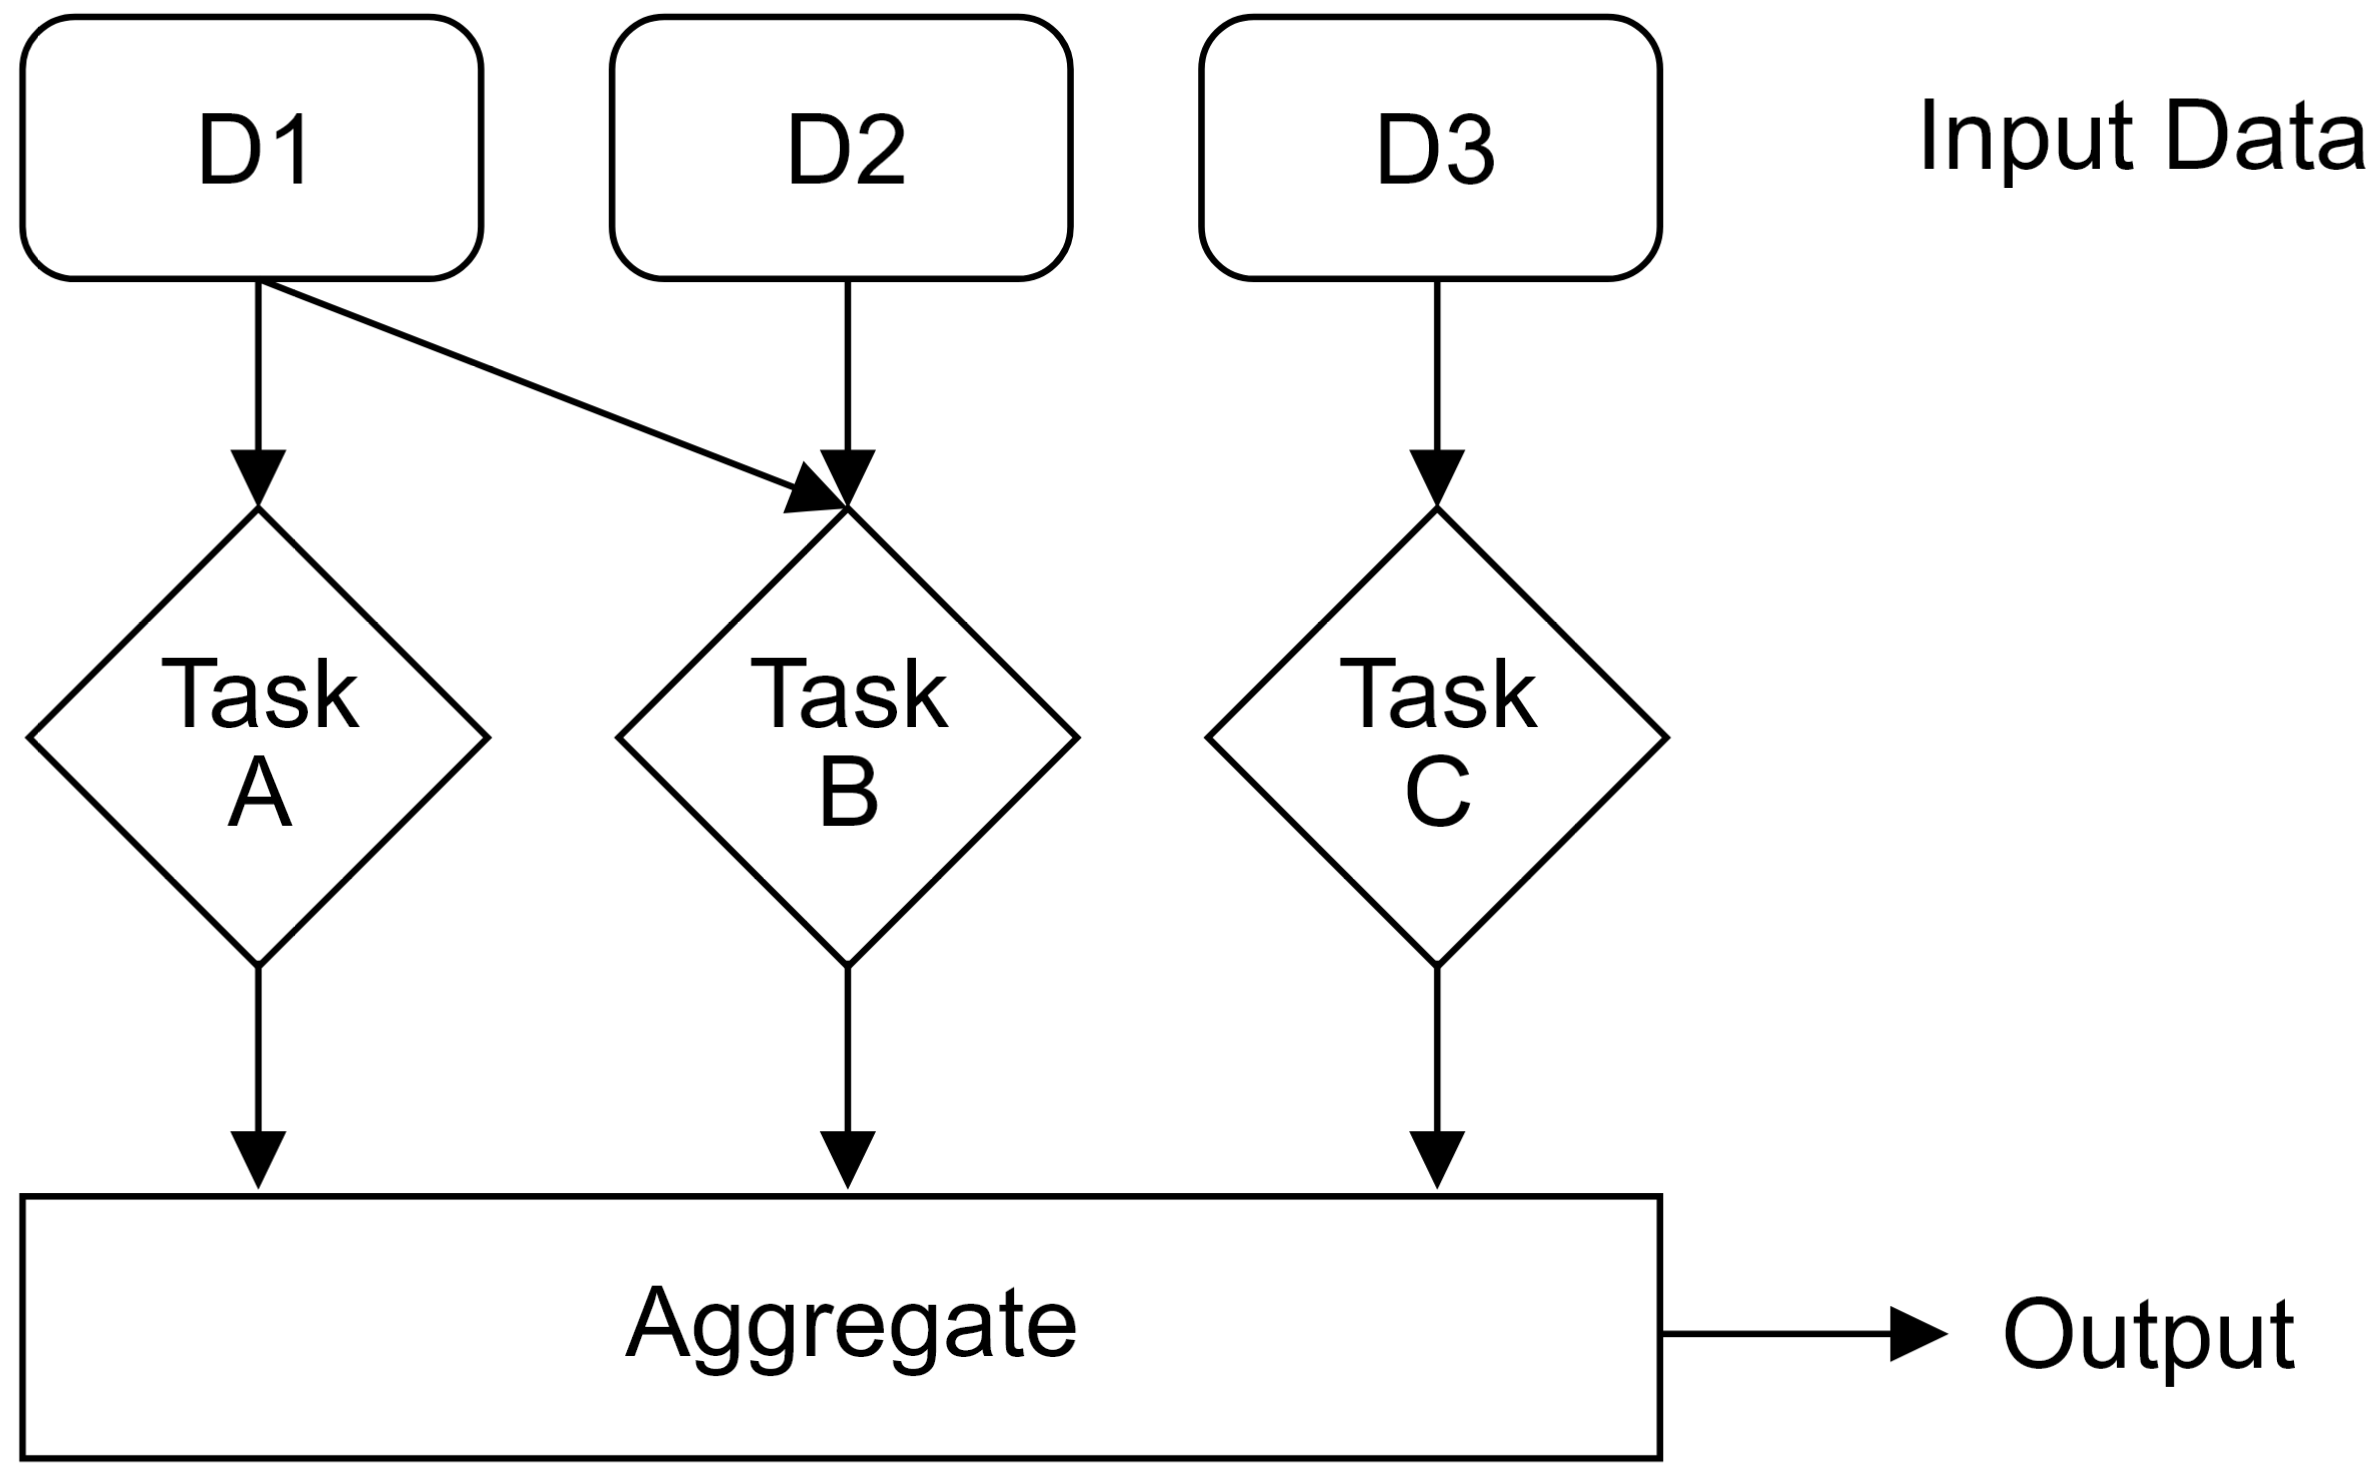
\includegraphics[width=.5\linewidth]{./Sections/rpc_2/tpar.png}
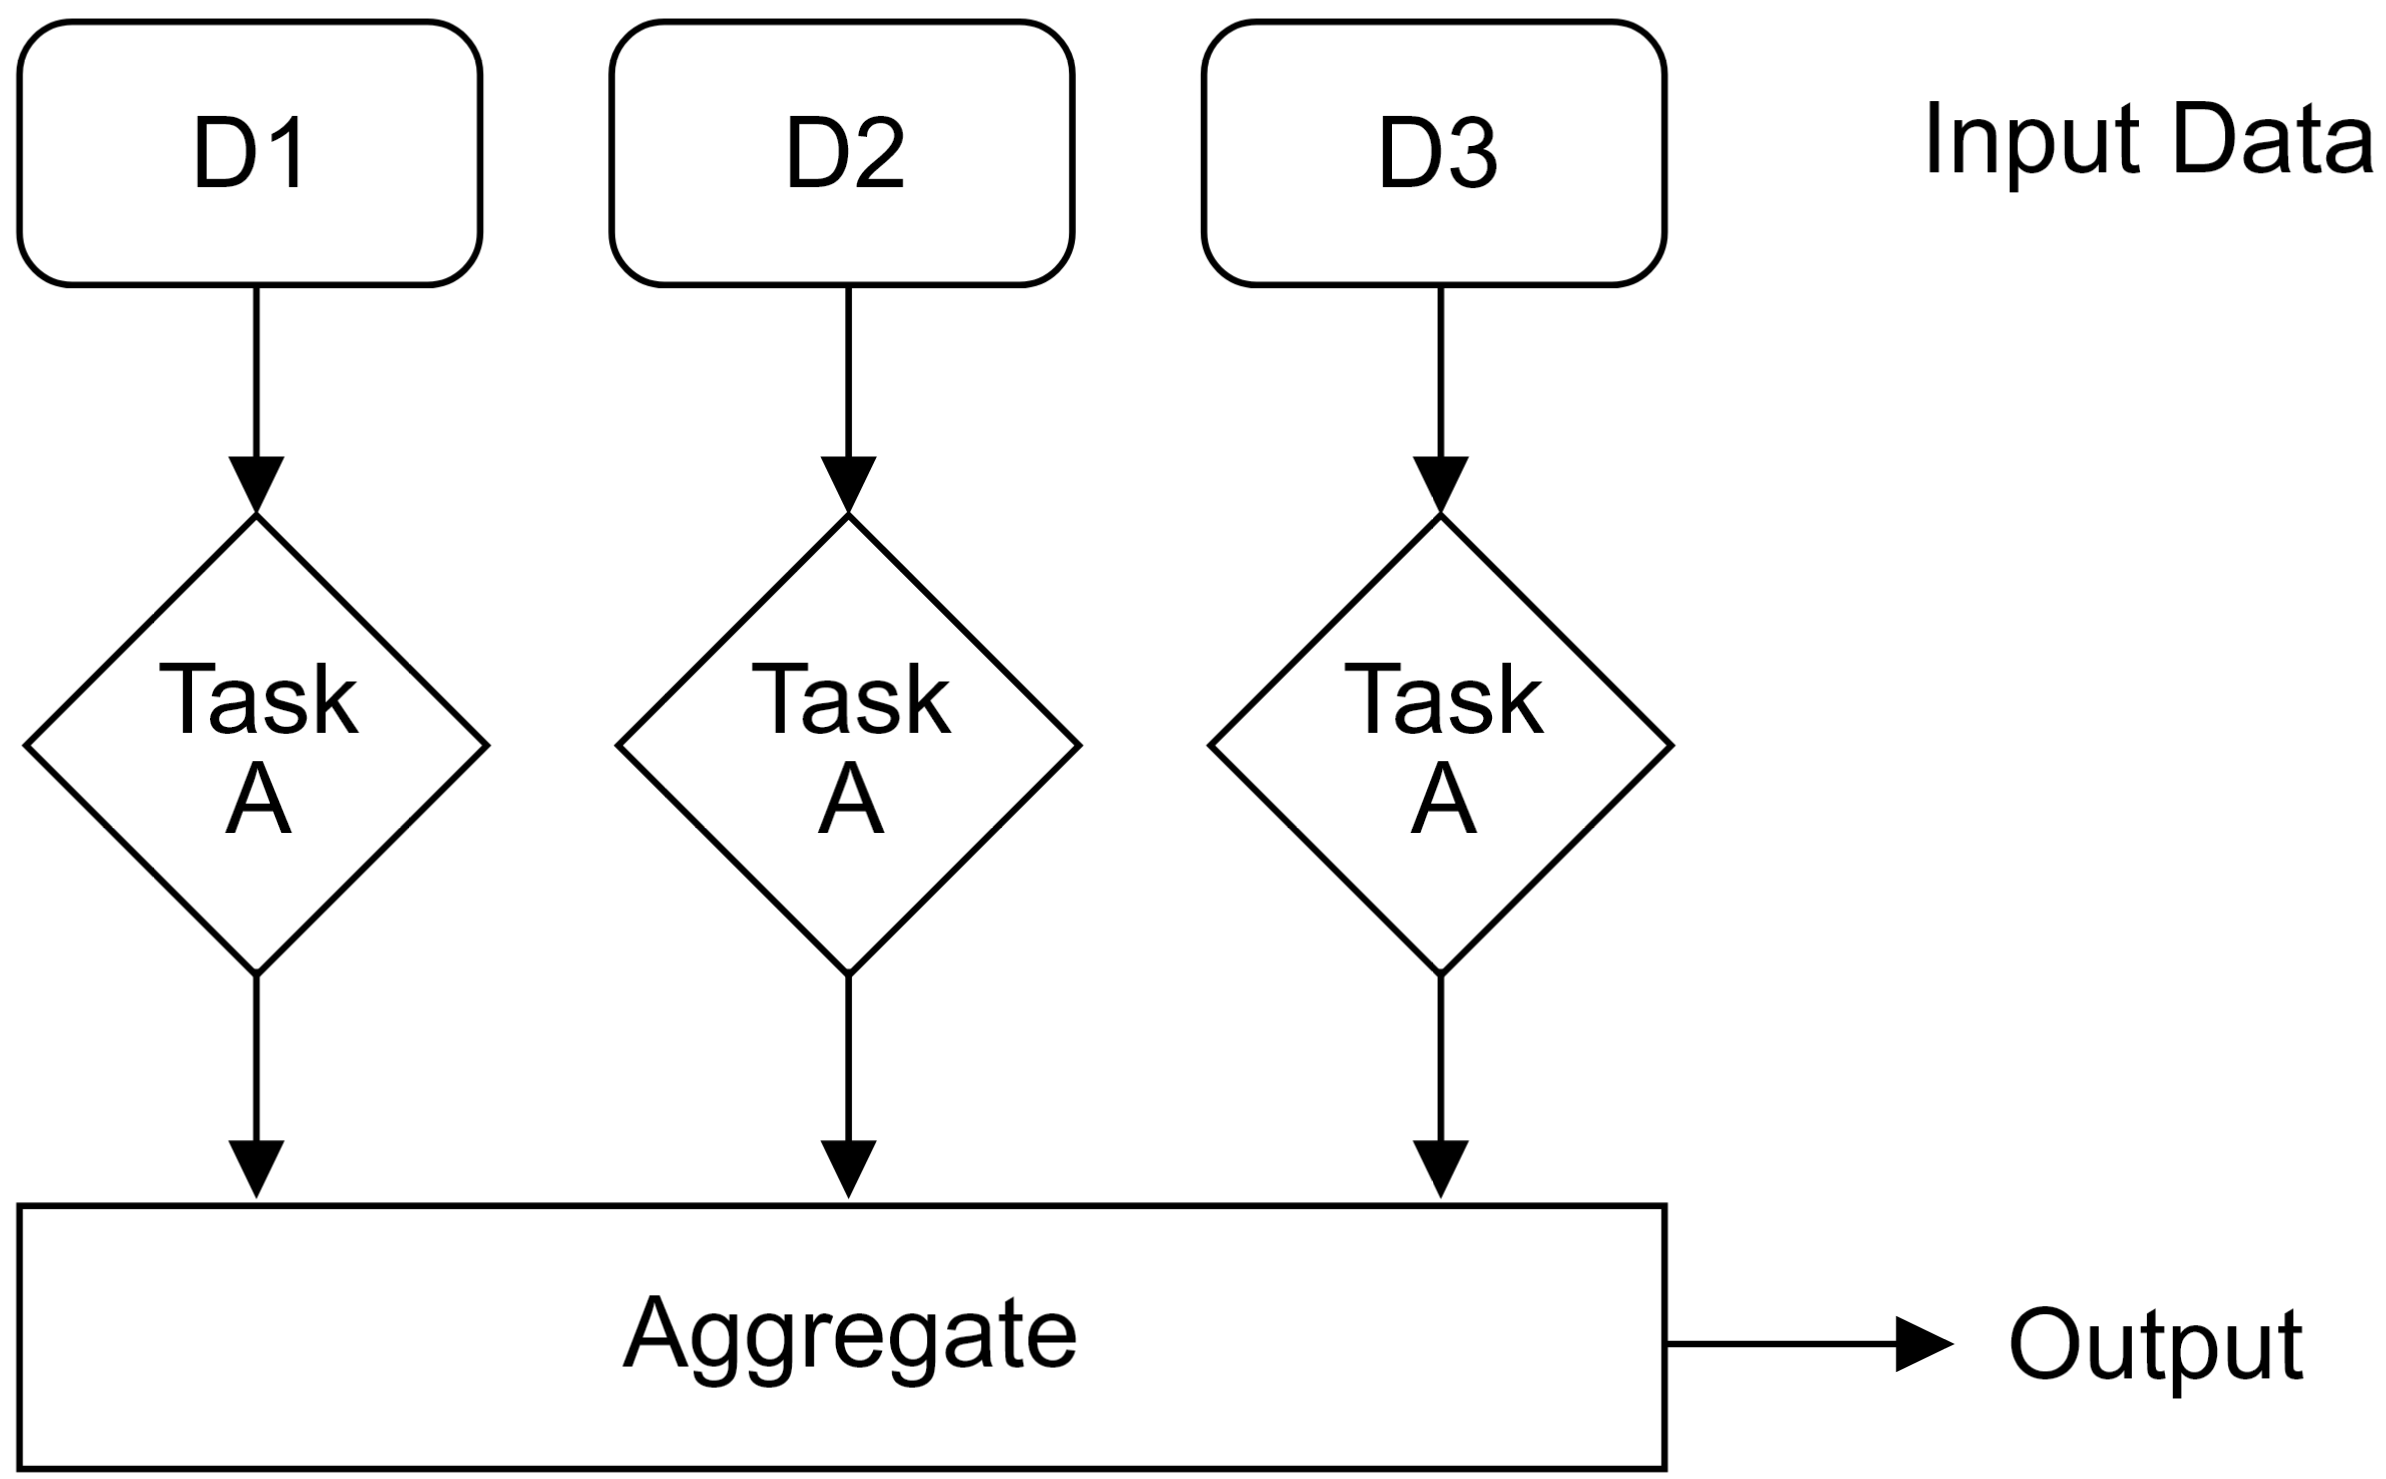
\includegraphics[width=.5\linewidth]{./Sections/rpc_2/dpar.png}\\
\noindent
\rule{\linewidth}{0.4pt}\\
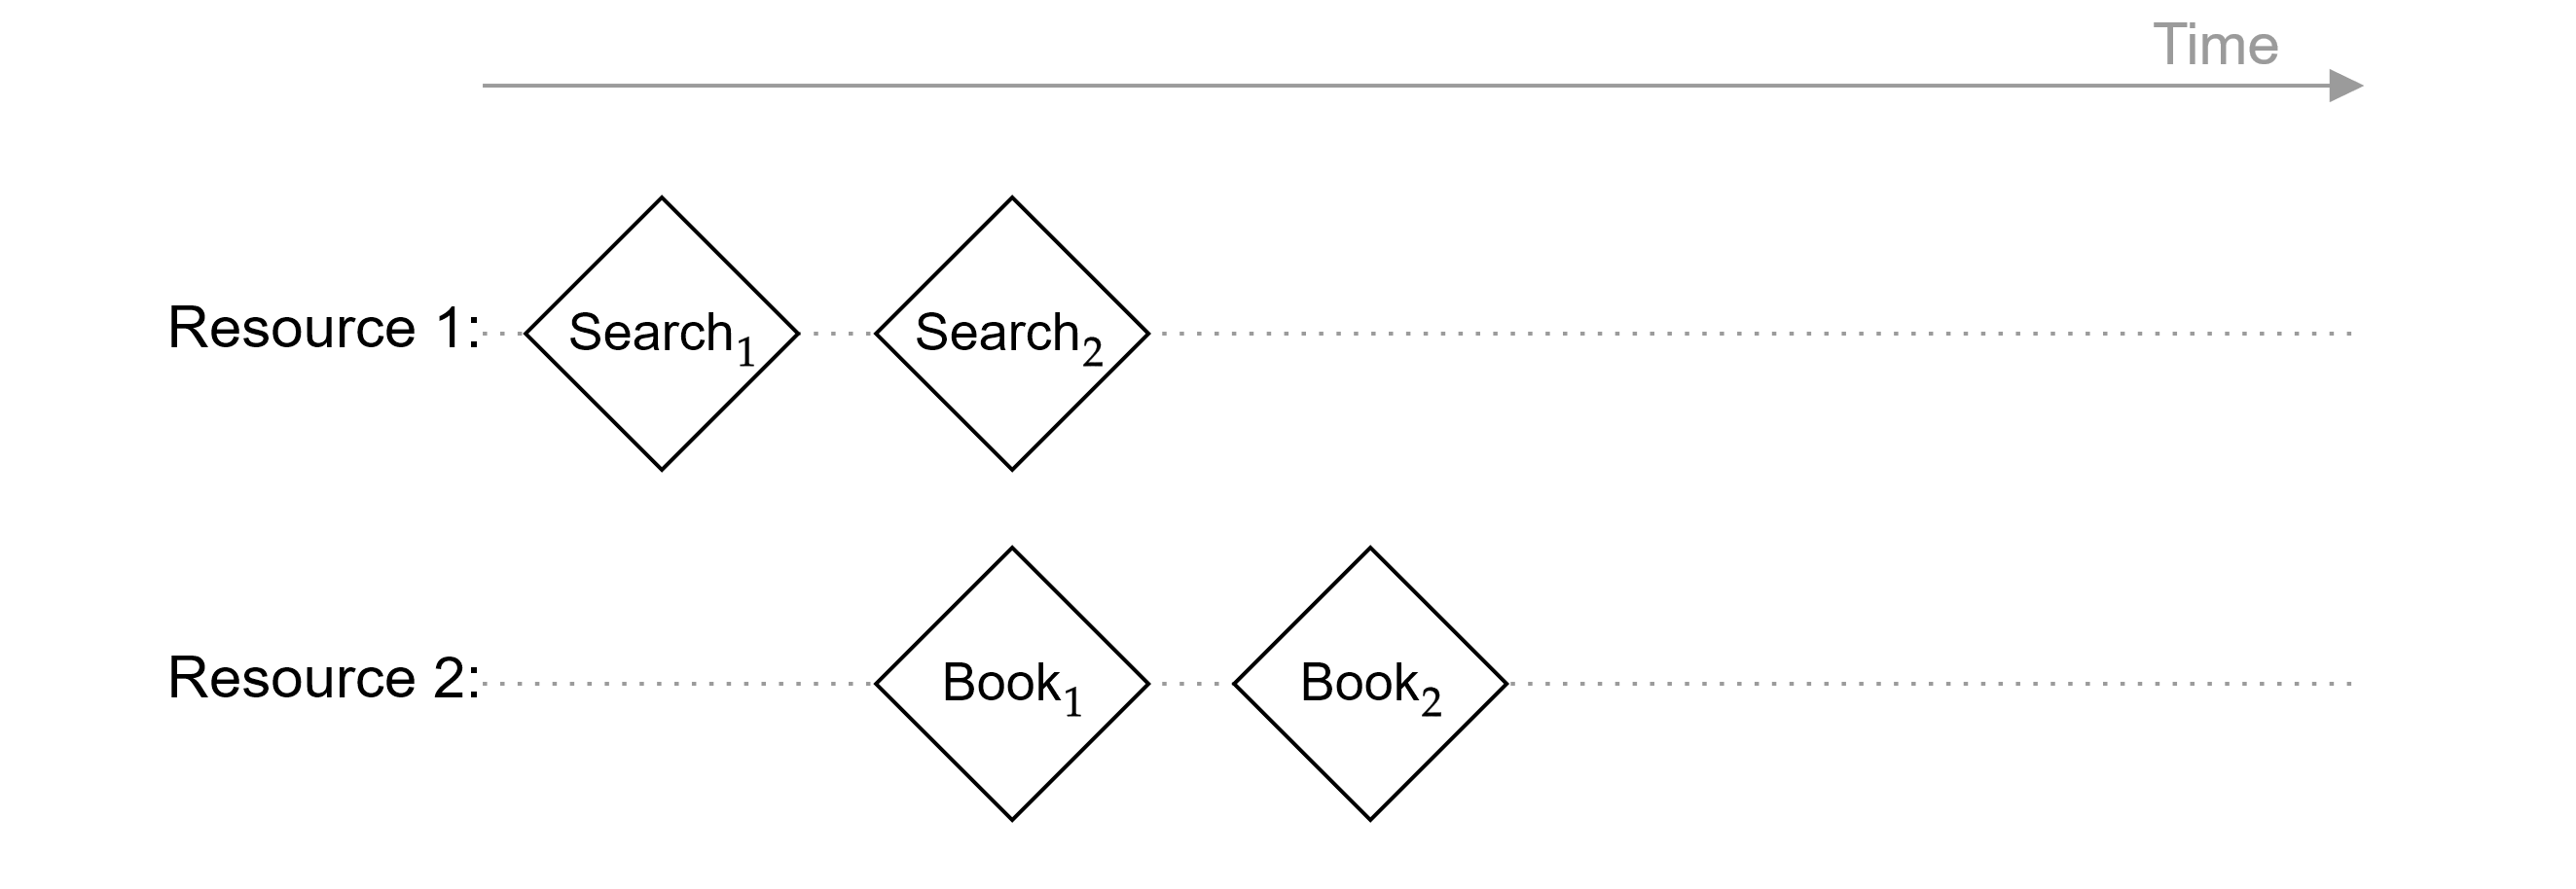
\includegraphics[width=\linewidth]{./Sections/rpc_2/ppar_2.png}
\noindent
\rule{\linewidth}{0.4pt}\\
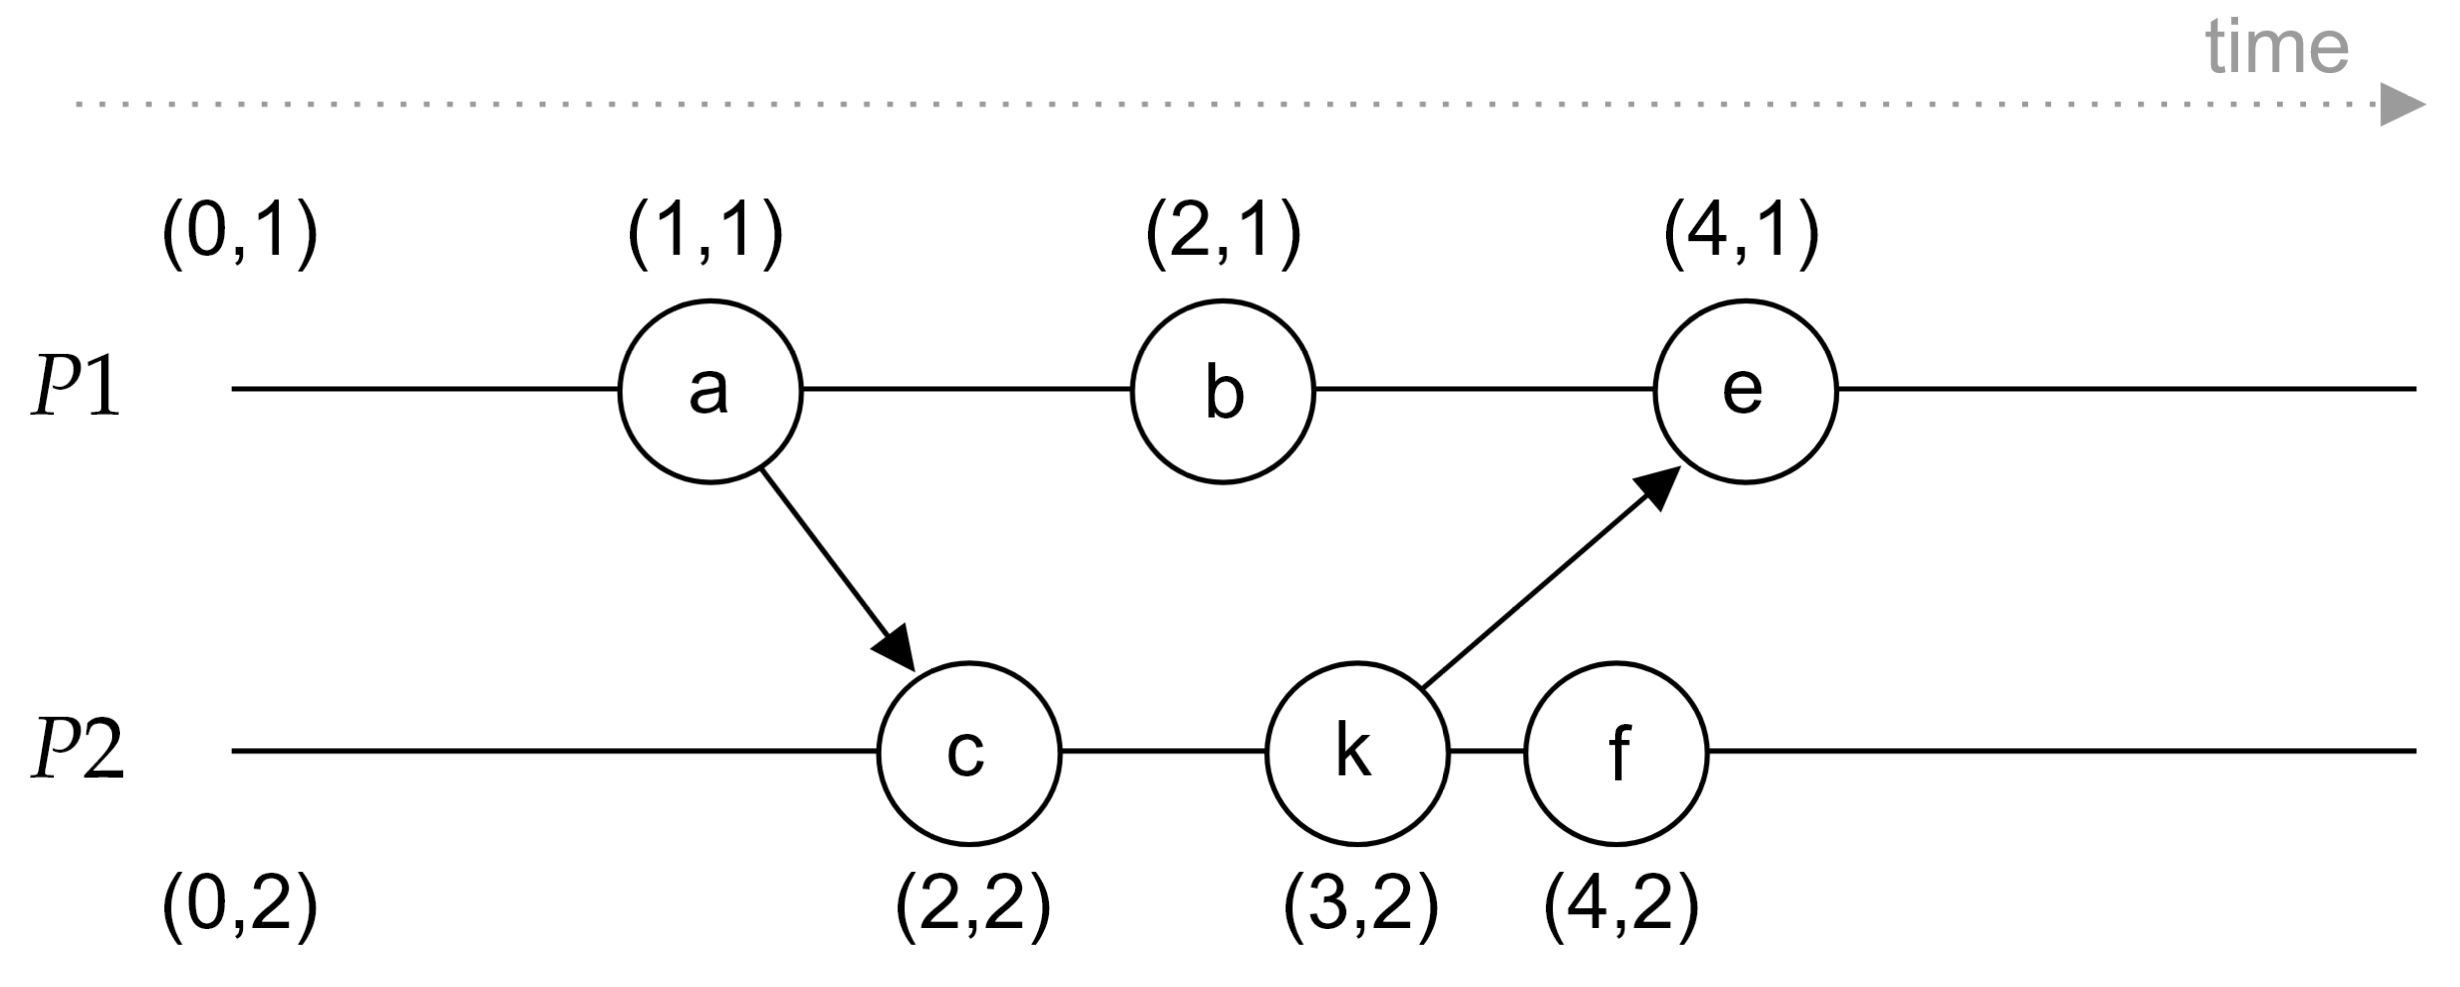
\includegraphics[width=\linewidth]{./Sections/time/lamport.png}
\noindent
\rule{\linewidth}{0.4pt}\\
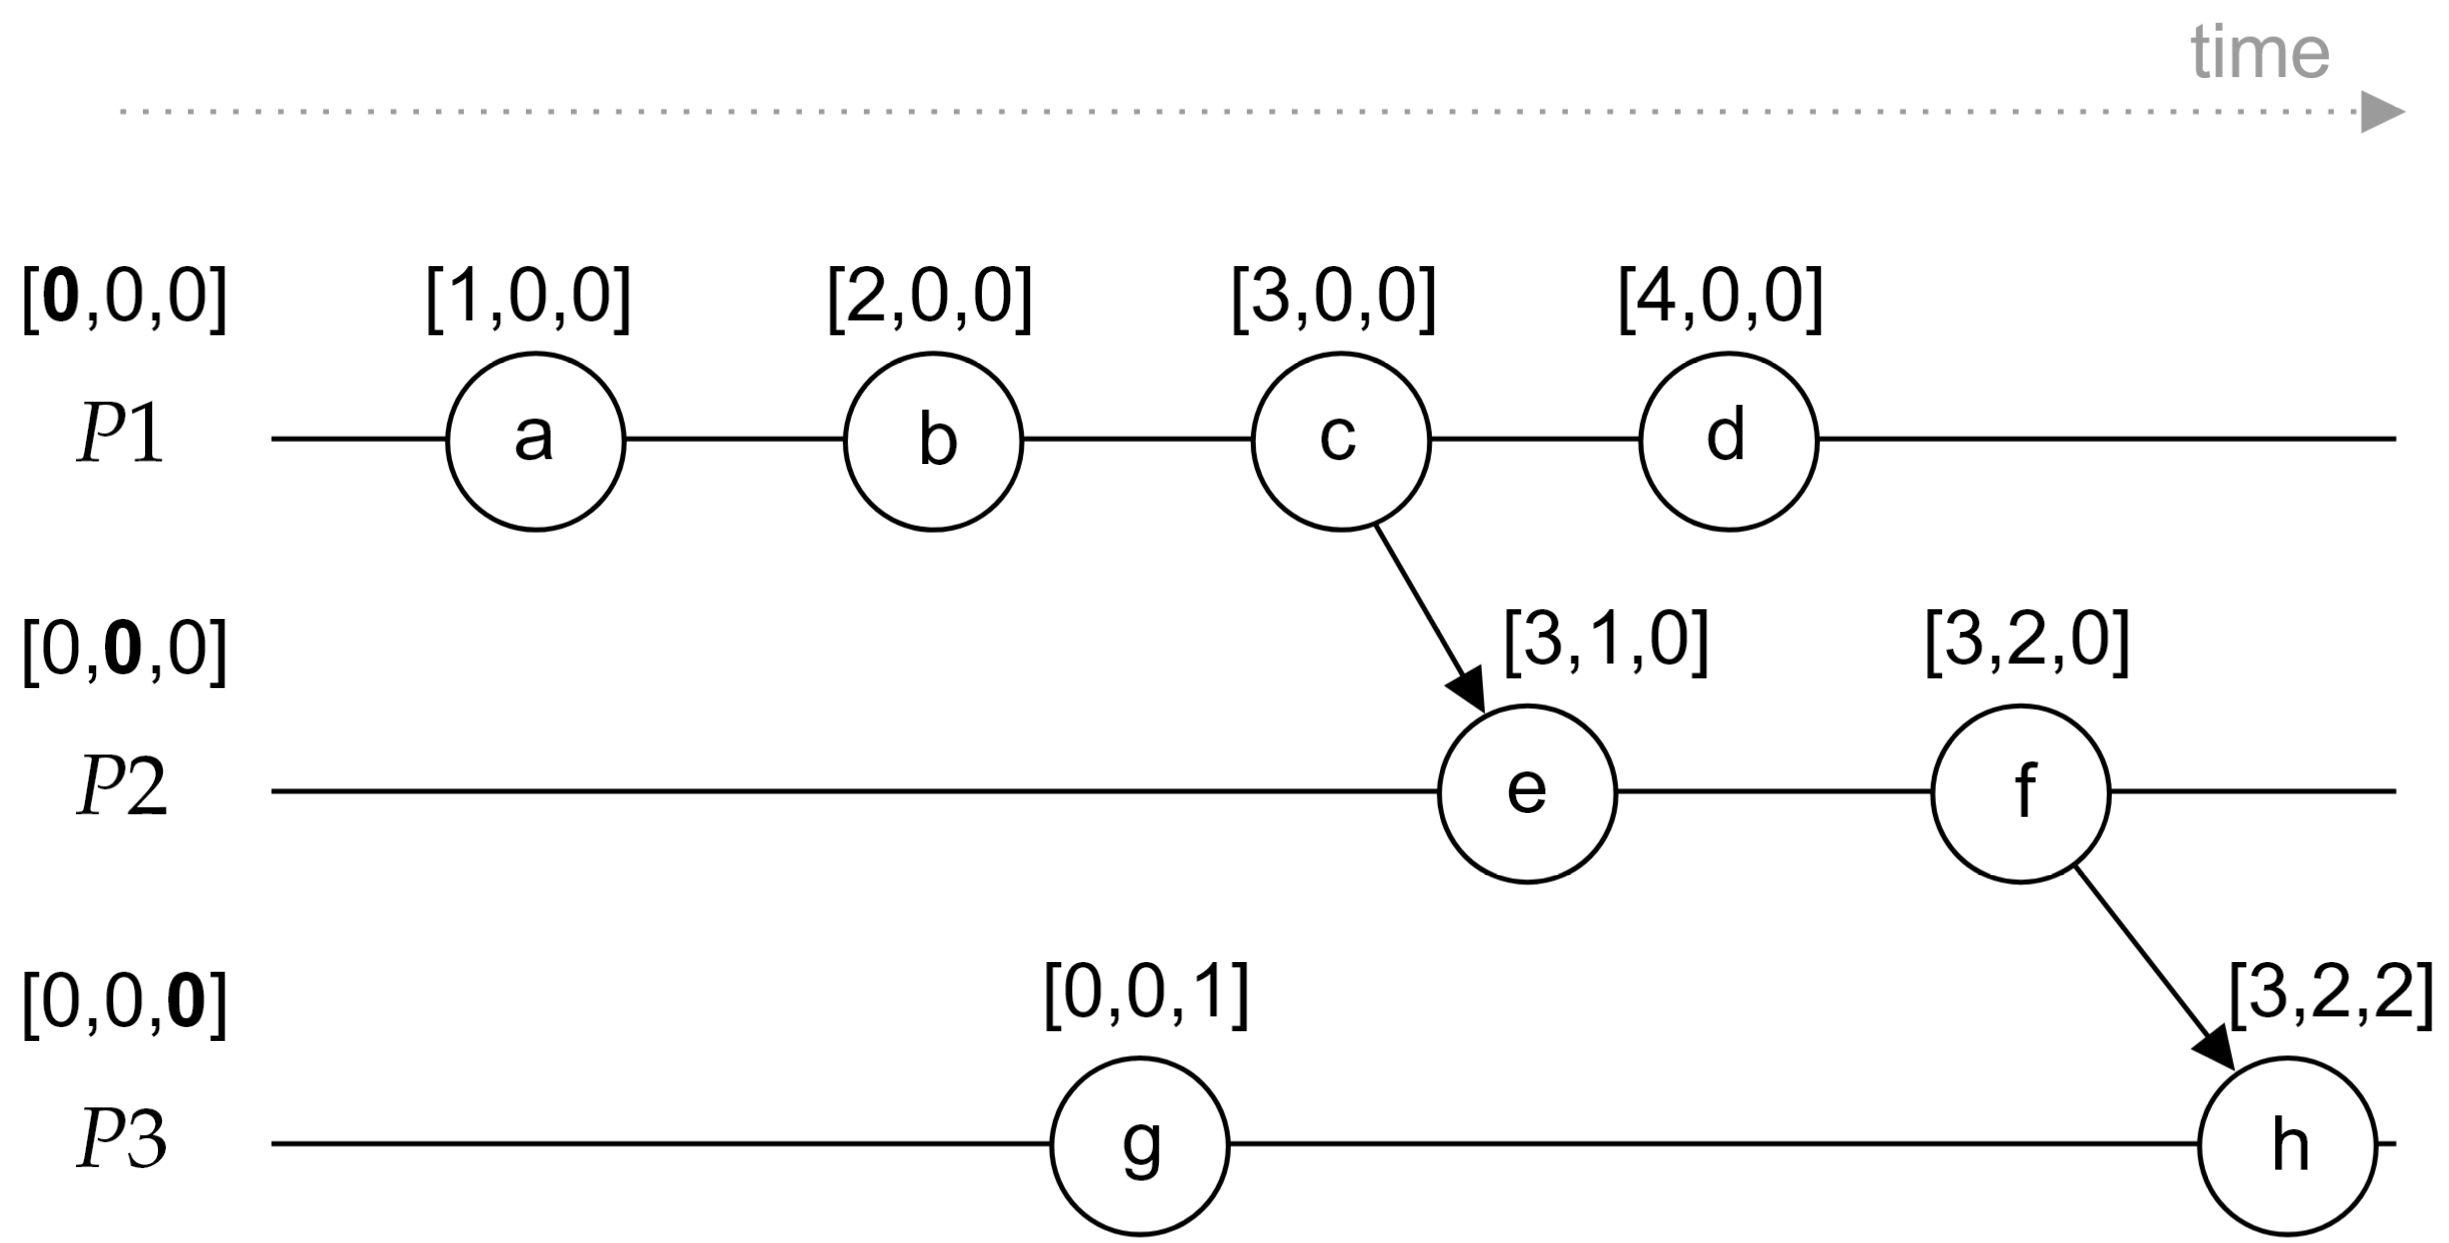
\includegraphics[width=\linewidth]{./Sections/time/vector.png}
\end{multicols}


\newpage

\begin{multicols}{2}
    
    \noindent
    \textbf{Snapshots:} Consistent snap., captures causal dependencies, if 
    $e_1 \to_r e_2$, and $e_2$ is in the snap., $e_1$ must also be present (otherwise it's inconsistent). If in the 
    snap., $e_1$ sent a message to $e_2$, and $e_2$ is not in the snap., replay the message on snap. recovery.
    \textbf{Chandy-Lamp.Snap:} Alg. for capturing consistent snaps. Reqs: No failures, FIFO channels, Strongly conn. graph, Single initiator.
    (1) Marker sent to all out-chans., record local state. (2) On marker retrieval, block (empty) the chan. from which it came. Record local state, except for empty chans. Send marker to all out-chans.
    (3) Completion, When all processes have received and sent a marker, the snapshot is complete.
    (every processes' incoming channel is empty).---\textbf{Replication}---
    \textbf{Def:} Maintaining multiple copies of the same data across distinct nodes (machines), providing fault-tolerance, load-balancing, and availability.
    \textbf{Active vs. Passive Rep:} Active, client sends reqs. to all replicas, must process in FIFO order. Passive, client sends reqs. to one replica (primary), which propagates to others (backups).
    \textbf{State vs. Req. Rep:} State Rep., forwards the entire state to backups. Request Rep., forwards individual reqs. to backups.
    \textbf{Primary Commit:} Client$\to$Primary$\to$Backups$\to$Primary$\to$Client (Commit Point).
    \textbf{Arbitrary Serv. (CFG):} The Configuration Service Provider (CFG) ensures a controlled \textbf{failover} (switching to backups) in the event of a primary failure.
    \textbf{Chain Rep:} An ordered chain of $s_n$ replicas, writes propagate from $s_1$ to $s_n$, where $s_n$ reports back to the client. Reads speak directly with $s_n$. For any failover, the next adjacent successor takes over.---\textbf{Consensus} (\ref{sec:raft})---\textbf{State Machine:}
    Processes a seq. of inputs from a log, saving them in state. \textbf{Rep. State Machine:} Replicated logs across multiple machines, the processing of 
    which is deterministic, generating the same state.\textbf{Consensus Model:} facilitates agreement of replicated logs between replicas.
    \textbf{Raft:} A consensus algorithm, with a central leader elected by the cluster in monotonically increasing terms. Liveliness is measured by periodic heartbeats, if the leader
    isn't reachable, followers, run for election. Split votes are dealt with the current candidates by timing out again (new timeout). Log Matching Property: Same index and term implies, same command and previous indexes are identical.
    Log Correction: The leader will find the index of the first mismatch, then overwrite the followers entries with its own. Leader Completeness: All proceeding leaders must have all committed entries of the previous leader.
    Leaders may only commit entries from their term. Candidates are rejected if they have a lower term, shorter log. Timings: $heartbeatReceipt \ll electionTimeout \ll failRate$. 
    Cluster Reconfiguration: A joint consensus reconfiguration follows two phases: (1) propagate mix config of old and new, (2) propagate new config, which includes new servers or deletions. New servers
    enter with empty logs. Log Compaction/Snapshotting: Servers independently take snapshots, which truncates all committed logs, storing the last committed log index, term, and state (key-value pairs).
    Clients are always redirected to the leader. 2ReplaysSnap. Primary \& Chain Rep.\\
    \noindent
    \rule{\linewidth}{0.4pt}\\
    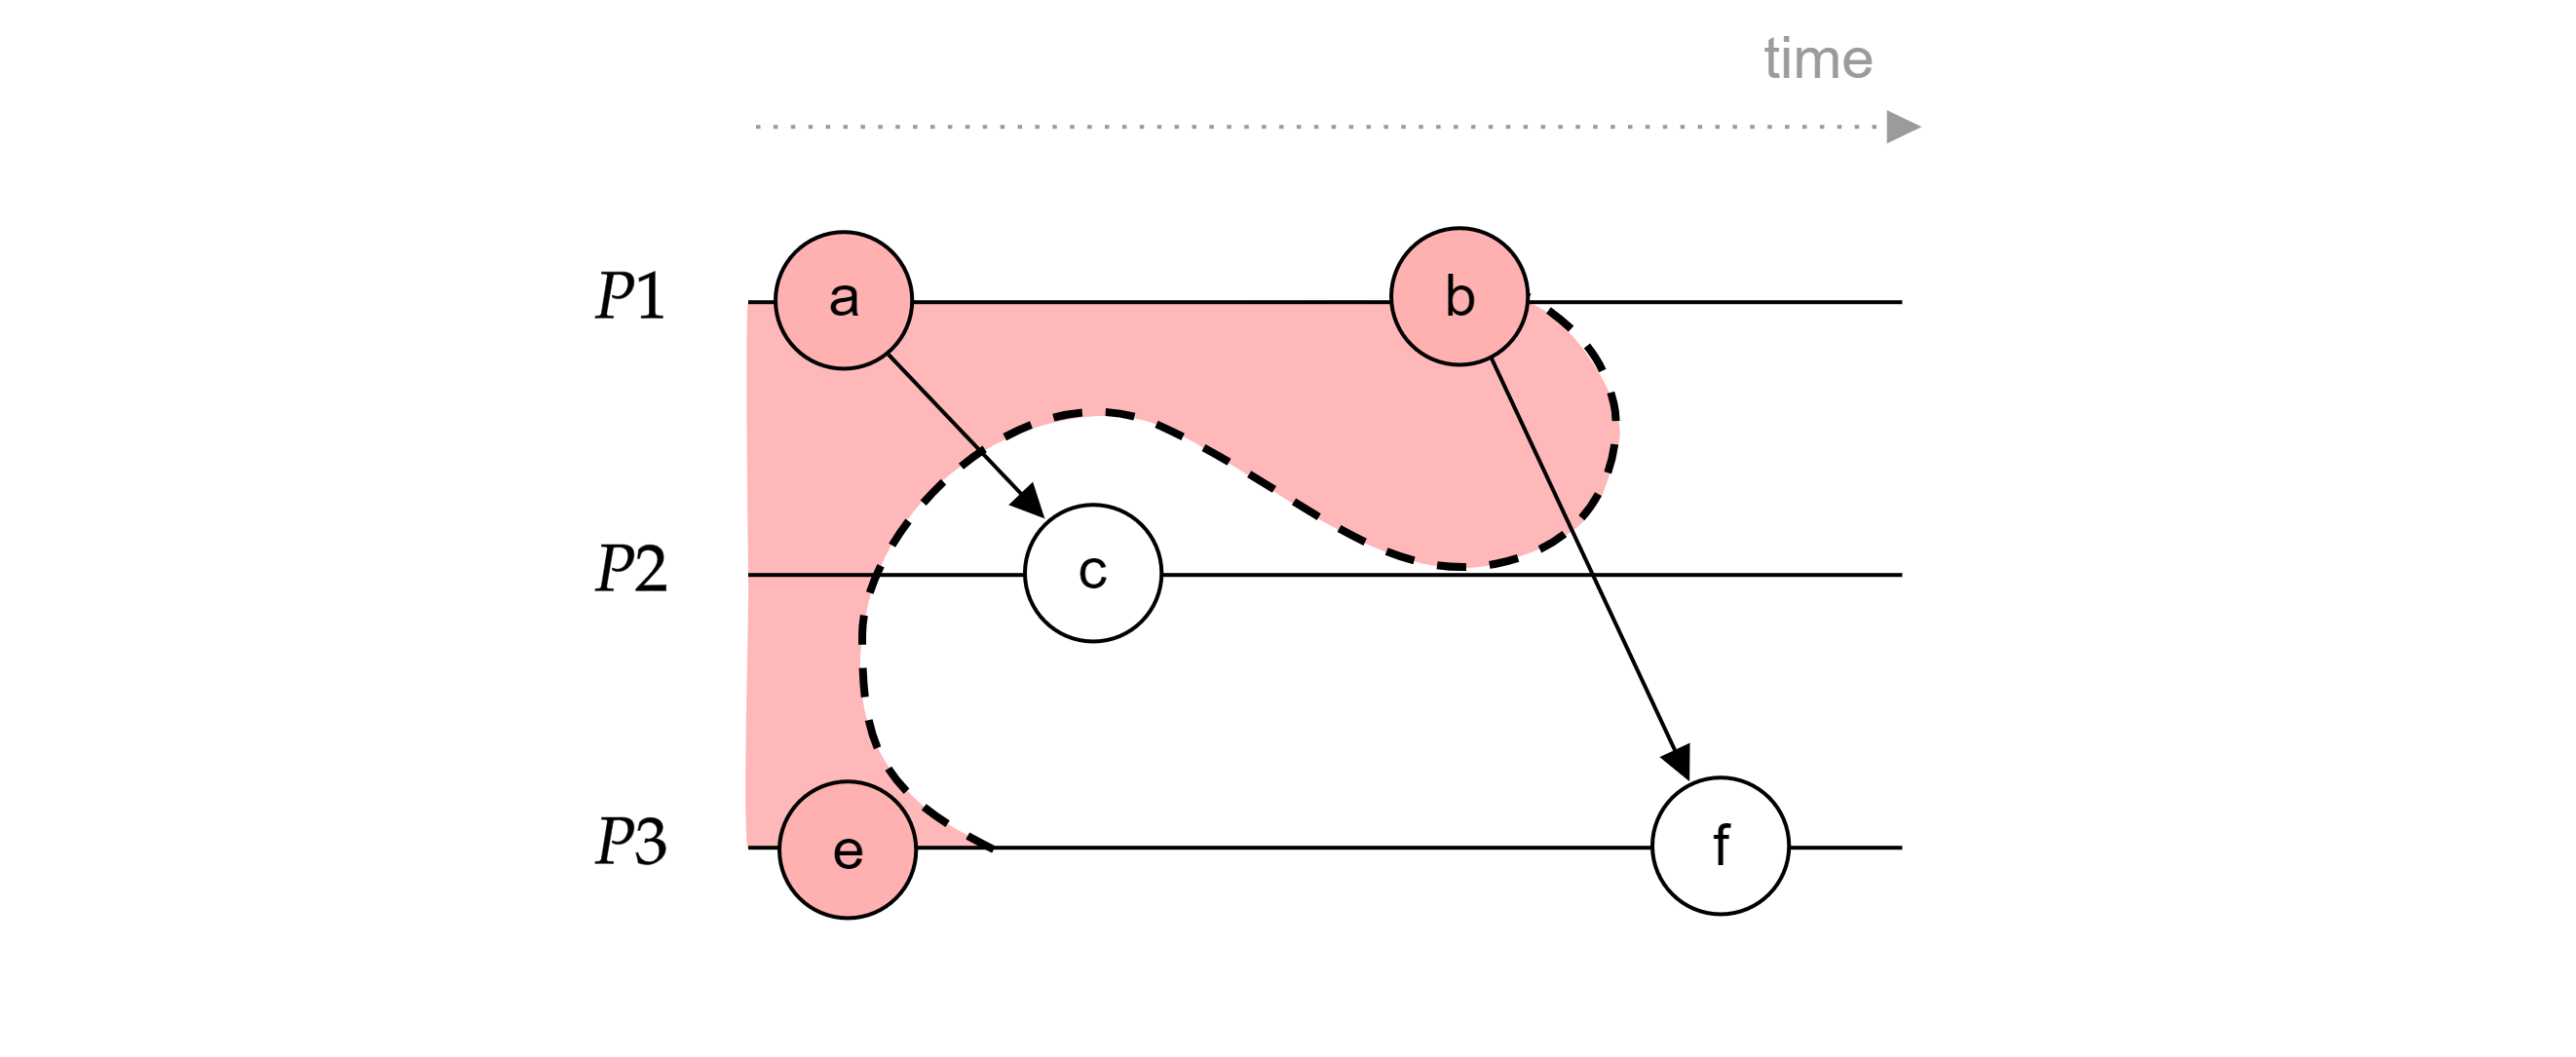
\includegraphics[width=\linewidth]{Sections/snap/snap_2.png}\\
    \vspace{-2.5em}
    \noindent
    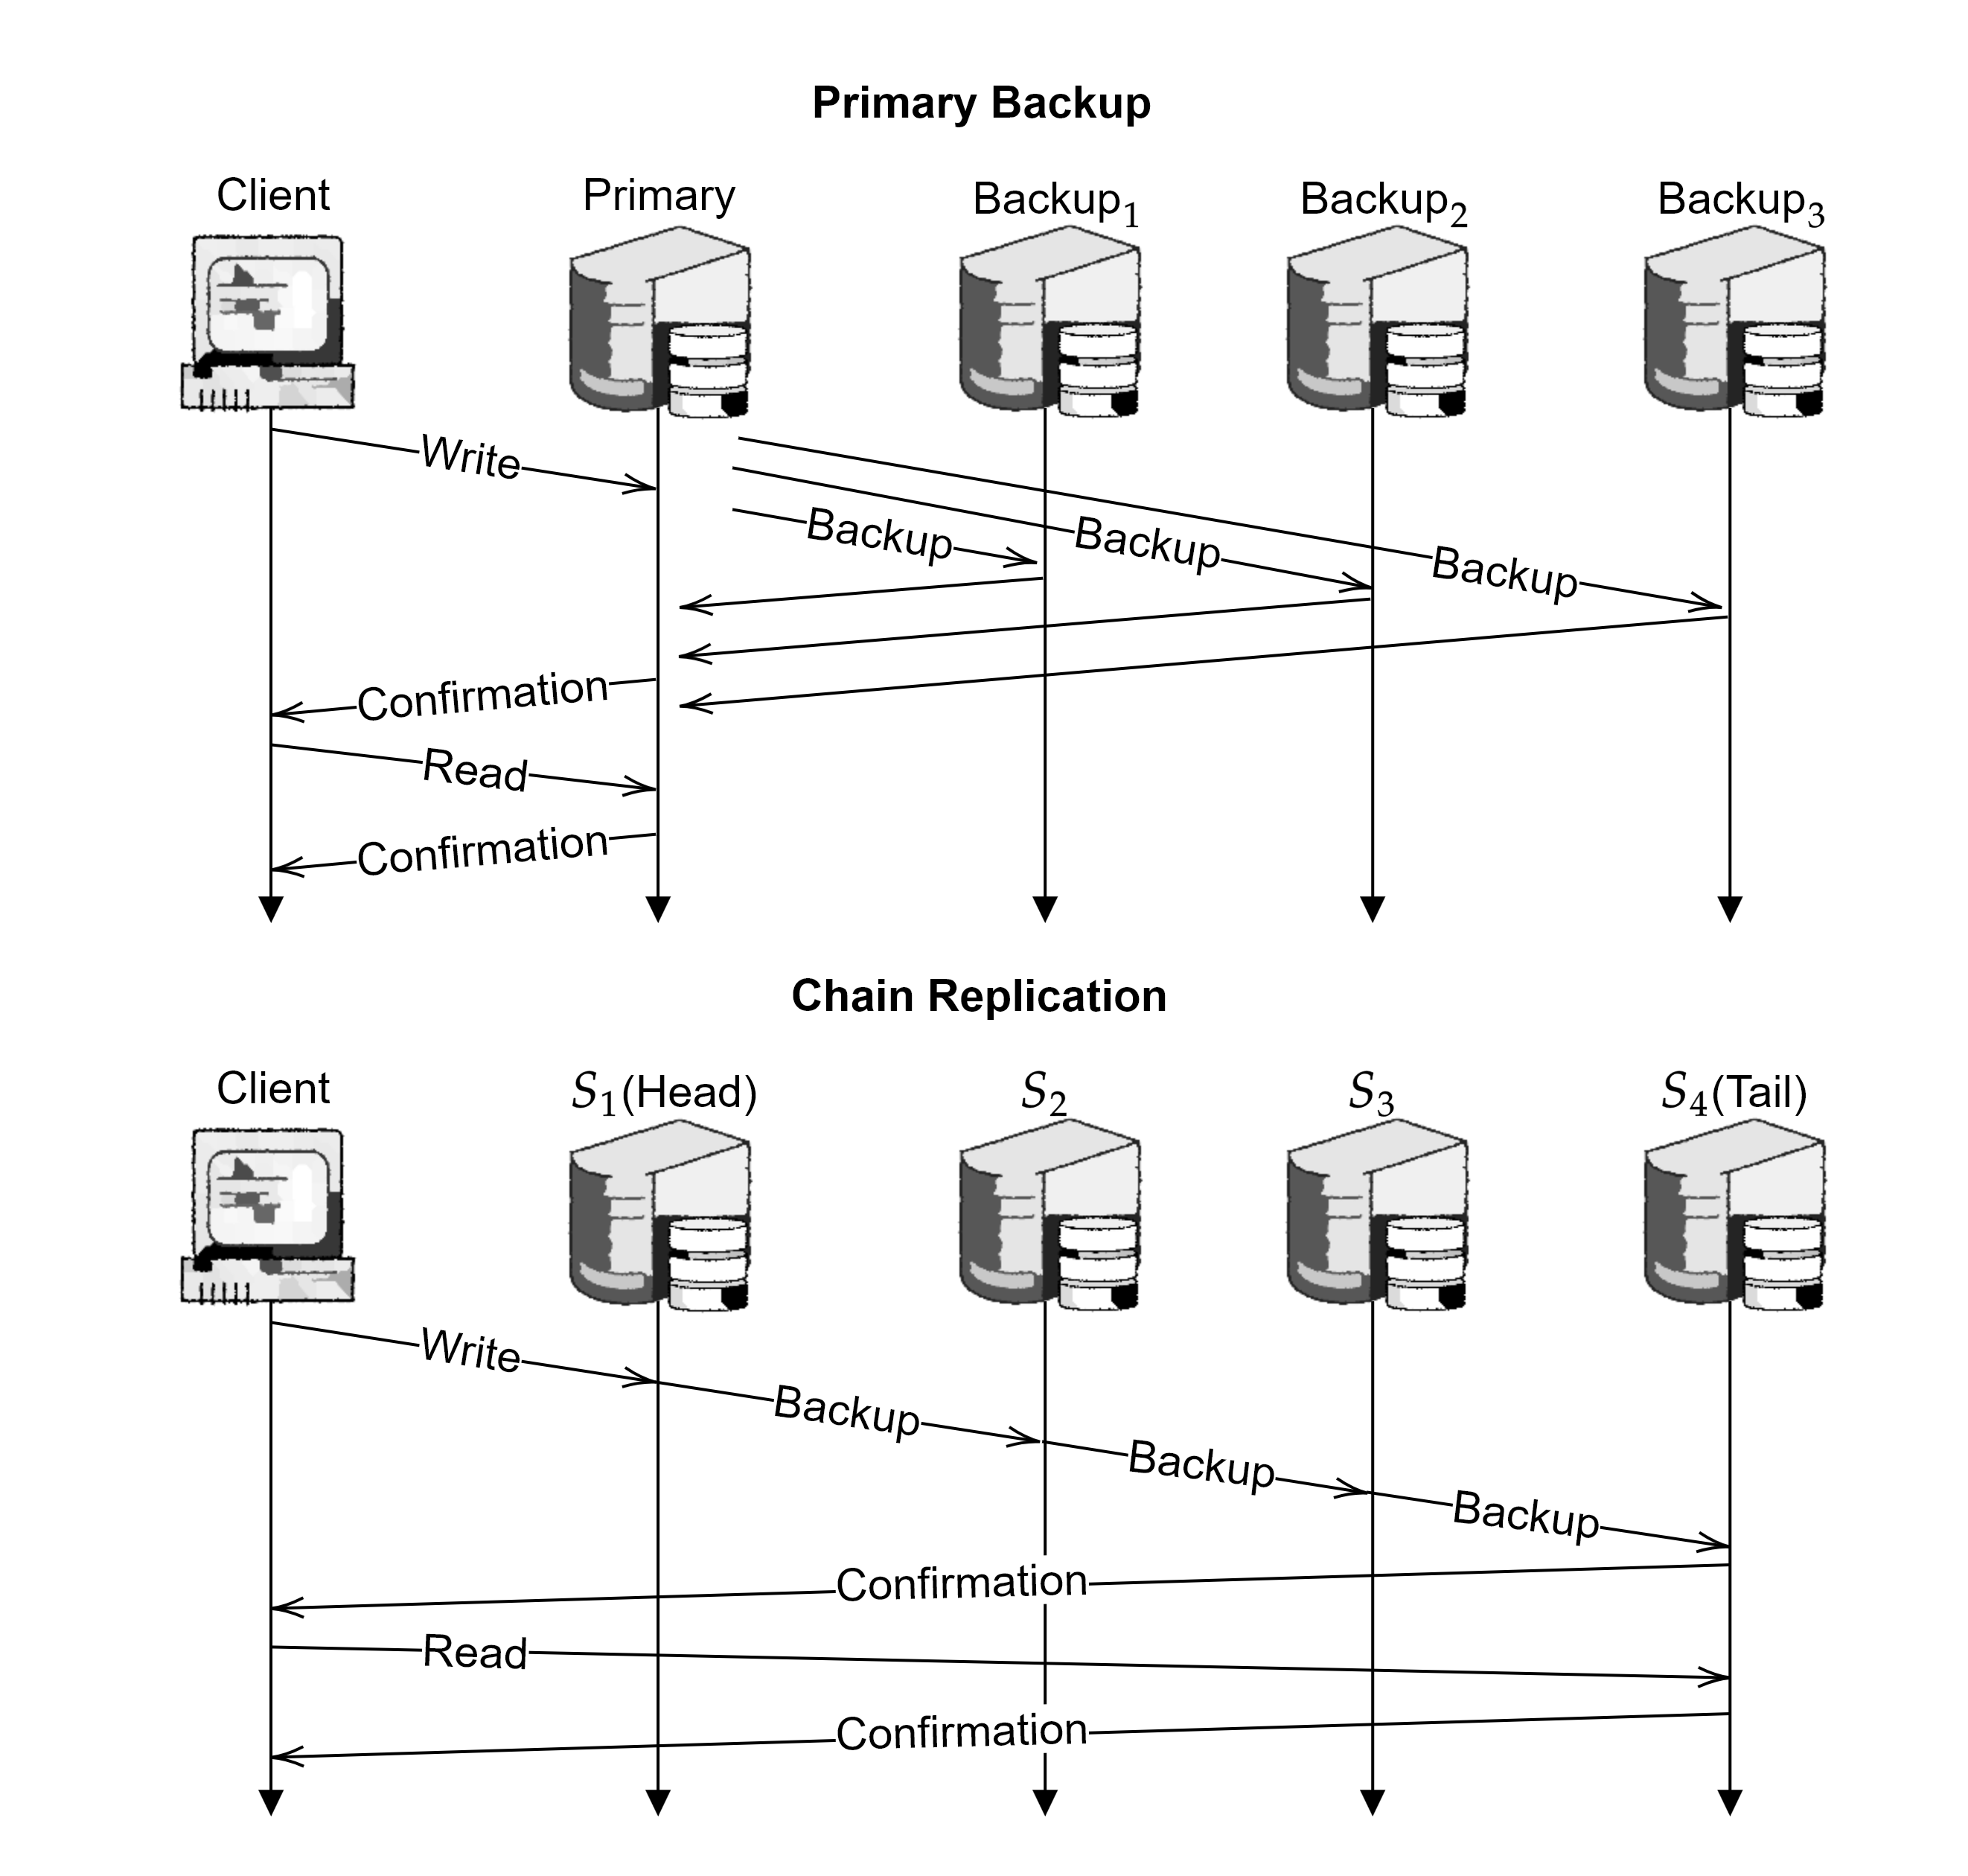
\includegraphics[width=\linewidth]{Sections/rep/comp.png}\\
    
\end{multicols}

\newpage 

\begin{multicols}{2}

\noindent
---\textbf{Failure Model Hierarchy} (\ref{sec:failures})---Crash-Stop: Process halts, cannot resume (undetectable) $\subset$ Omission: Process fails to properly communicate $\subset$ 
Crash-Recovery: Process halts, but can recover $\subset$ Byzantine: Process exhibits arbitrary or malicious behavior.---\textbf{Consistency Models} (\ref{sec:consist})---\textbf{Def:} A distributed system's method on validating operation orderings on shared data.
\textbf{Global Total Order:} Order of observable events agreed upon by all clients. \textbf{Strong Consistency (Str):} The client observes nodes agree on order execution (all node reads appear to be identical).
\textbf{Weak Consistency (Wck):} The client temporarily observes that nodes disagree on shared data values.
\textbf{Linearizability (Str):} Global Total Order with respect to real-time ordering (operation time intervals unmovable, but execution choice within them are). E.g., Raft leader-commit (happy-path) and Chain Replication.
\textbf{Sequential (Str):} There is some Global Total Order found when shifting operation time intervals.
\textbf{Causal Consistency (Wck):} Same as Sequential; However, clients may observe their own view on a Global Total Order.
\textbf{Eventual Consistency (Wck):} Given no new writes, replicas will eventually agree on the same value after some time.
\textbf{Causal Implications:} Linearizability $\implies$ Sequential $\implies$ Causal $\implies$ [First-In-First-Out (FIFO)/ Read-Your-Writes (RYW)].
\textbf{Release Consistency (Wck):} Push updates to all nodes after releasing the lock. 
\textbf{Lazy-release Consistency (Wck):} Push updates to the next node who acquires the same
lock.---\textbf{Transactions} (\ref{sec:occ})---\textbf{ACID:} Atomicity, no partial effects, all or nothing. Consistency,  A transaction takes the database from one valid state to another. 
Isolation, no interleaving of transactions.
Durability, transactions once committed, are permanent even after system failure.
\textbf{Serializability (Str):} Ensures the outcome of concurrent transactions is the same as if they executed in some serial (sequential) order. Differs from 
linearizability, which deals with real-time ordering of single tasks, as opposed to whole jobs. 
\textbf{Strict-Serializability (Str):} Serializability with real-time ordering; In particular, Serializability $\Longleftarrow$ Strict-Serializability $\implies$ Linearizability.
\textbf{Optimistic Concurrency Control (OCC):} Assumes conflicts are rare, proceeds without locking. (1) Prepare the transaction on all nodes, (2) Tell the coordinator to execute, validate the outcome, (3) Commit if Serializable, abort otherwise (isolation).
\textbf{Timestamping OCC:} Helps with distributed OCC agreement on separated data, but aborts unnecessarily.
\textbf{Two-Phase Commit (2PC):} Ensures \textbf{atomicity}, (1) Prepare Phase: After client's request is received on all nodes, the Transaction Coordinator (TC) sends a prepare message to all nodes, awaiting YES votes. 
(2) Commit Phase: If all nodes reply YES, the TC requests for all nodes to commit. If any fail to reply, the TC is blocked, sending the commit request to that node indefinitely (can't abort after this point).
\textbf{3PC:} 2PC with an additional phase before the commit phase, ensuring people can commit (PreCommit Phase). If any nos or failure to respond in PreCommit, abort. If not 
partitioned, if the TC fails in the PreCommit phase, servers may attempt to reconcile with themselves about how to continue.
\textbf{Pessimistic Concurrency Control (PCC):} Assumes conflicts are likely and prevents them by ac-
quiring locks before any data access. It then preforms actions directly on shared data, ensuring
serializability and isolation. The locks are released after the transaction is completed. 3PC.

\noindent
\rule{\linewidth}{0.4pt}\\

\hspace{-1.5em}
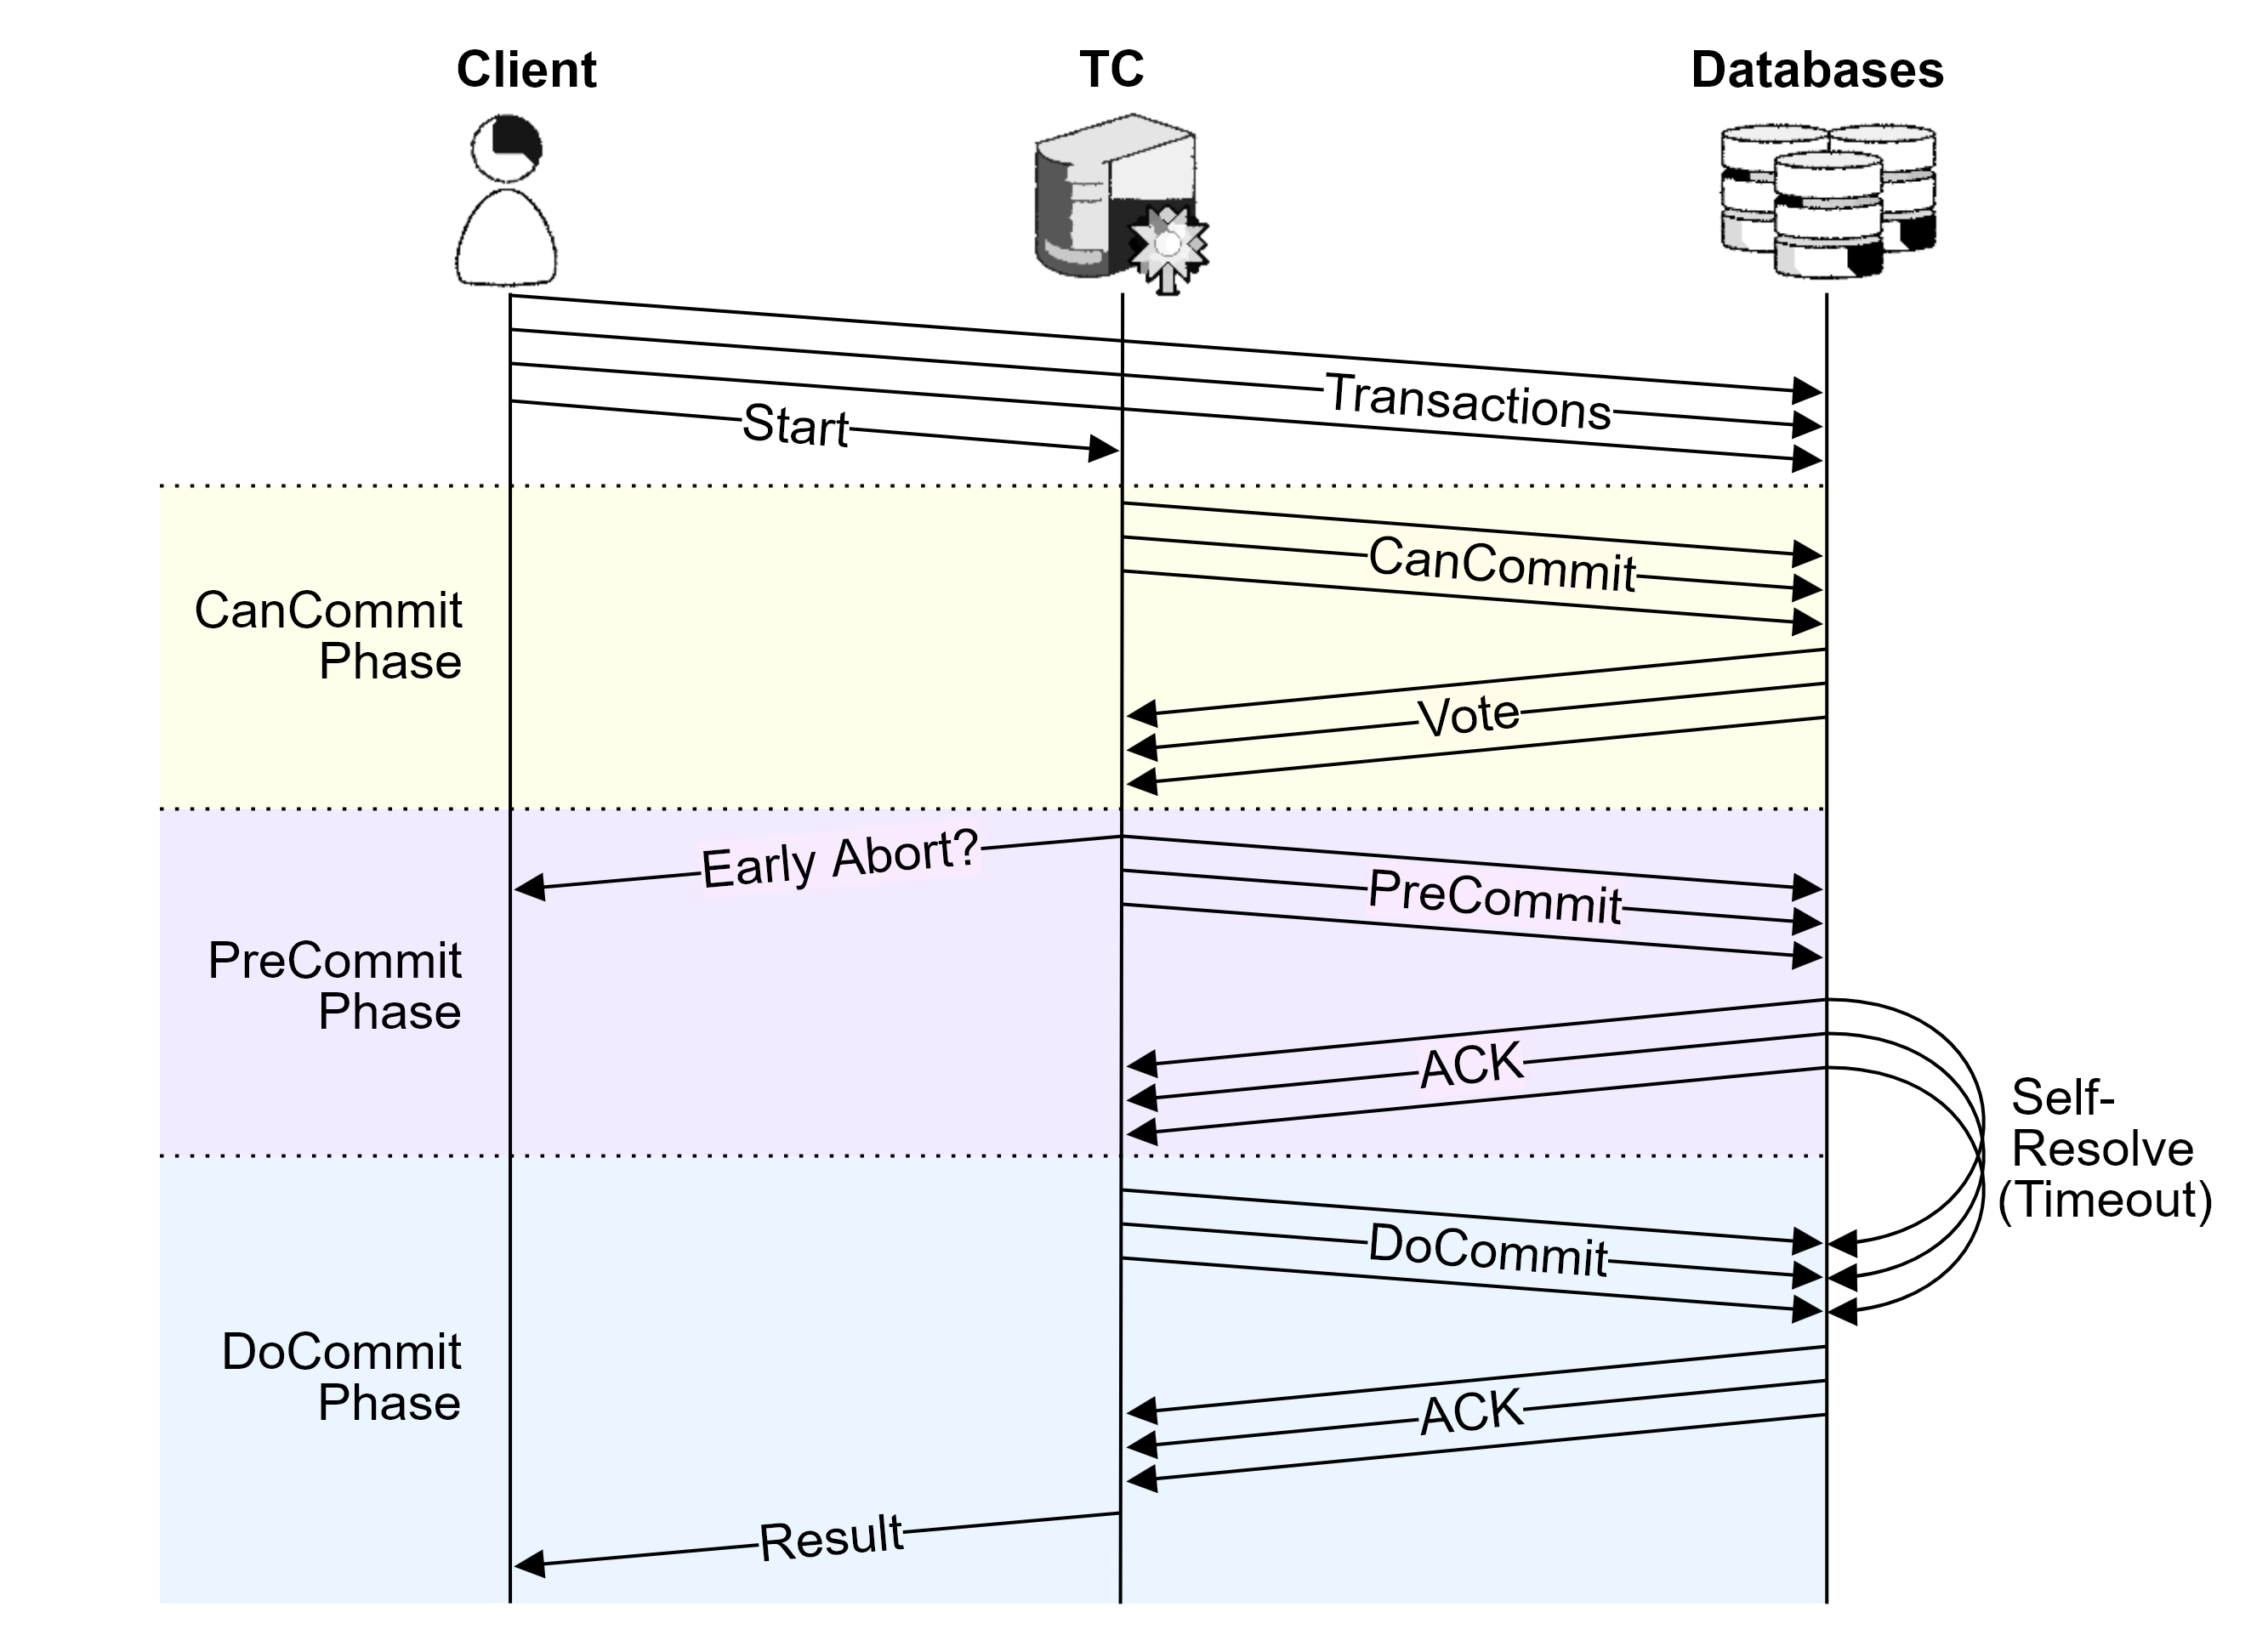
\includegraphics[width=\linewidth]{Sections/trans/3PC.png}\\

\end{multicols}

\newpage

\begin{multicols}{2}

\noindent
---\textbf{Distributed Shared Memory (DSM)} (\ref{sec:shared})---\textbf{Def (str):} A cluster which gives the 
illusion of a single shared memory space on a single machine, enabling multithreaded programs in a 
distributed setting. DSMs abstract away consensus and communication, opting to mimic virtual memory page primitives 
to communicate between nodes. \textbf{Sending Pages (Naive) (str):} Sending entire pages over the network is costly on bandwidth, but ensures consistency.
\textbf{Sending Page Diffs (TreadMark) (Wck):} Keep a versioning history of every change, upon request, send the diffs to the page, avoiding false sharing (unnecessary updates).
Versioning control is managed via vector clocks, which identify who made the changes (causal consistency). (1) Pages start as read-only (RO), which
many may access. (2) When one claims read-write (RW) access, it invalidates all other copies. (3) Upon request, a page diff is sent over the network,
the page now reverts to RO (at most one writeable copy). Weak consistency as per lazy-release style of data
sharing.---\textbf{Virtualizing} (\ref{sec:shard})---\textbf{Sharding:} Splitting a dataset into smaller chunks, called shards stored on multiple nodes. Multiple copies increases
safety. \textbf{Consistent Hashing:} Creates a hash ring of $2^m$ entries with keys of $m$-bit values. Servers 
are placed uniformly in multiple locations on a ring, serving for a range of
keys.
This helps with load balancing, as when one server goes down, the next clock-wise key ranges will help bare the load---\textbf{MapReduce:} (\ref{sec:mapreduce})---\textbf{Def:} Map: Takes a set of input key-value pairs and produces a set of intermediate key-value
pairs. Shuffle: this phase sorts the keys or hashes them (more efficient) into key bins that will be assigned to workers to reduce. Reduce: Takes an intermediate key and a set of values for that key, and merges them
into a smaller set of values. Given $W$ workers, $M$ mapping tasks, and $R$ reducing tasks, $W \gg N$ and $R \gg N$.  Data is split up and given 
to workers in partitions.
Map failure: Reassign the chunk, first one done is propagated. 
Reduce failure: Reassign the partition, they write to the same location (e.g., ``/filepath/final\_data/id'').
Coordinator failure: Restart the entire MapReduce job. Failures are not recoverable, and are assumed to be rare.
Slow workers (stragglers), will always be a bottleneck.
MapRed. Lin. Even. $\neg$Caus.


\noindent
\rule{\linewidth}{0.4pt}\\

\hspace{-1.5em}
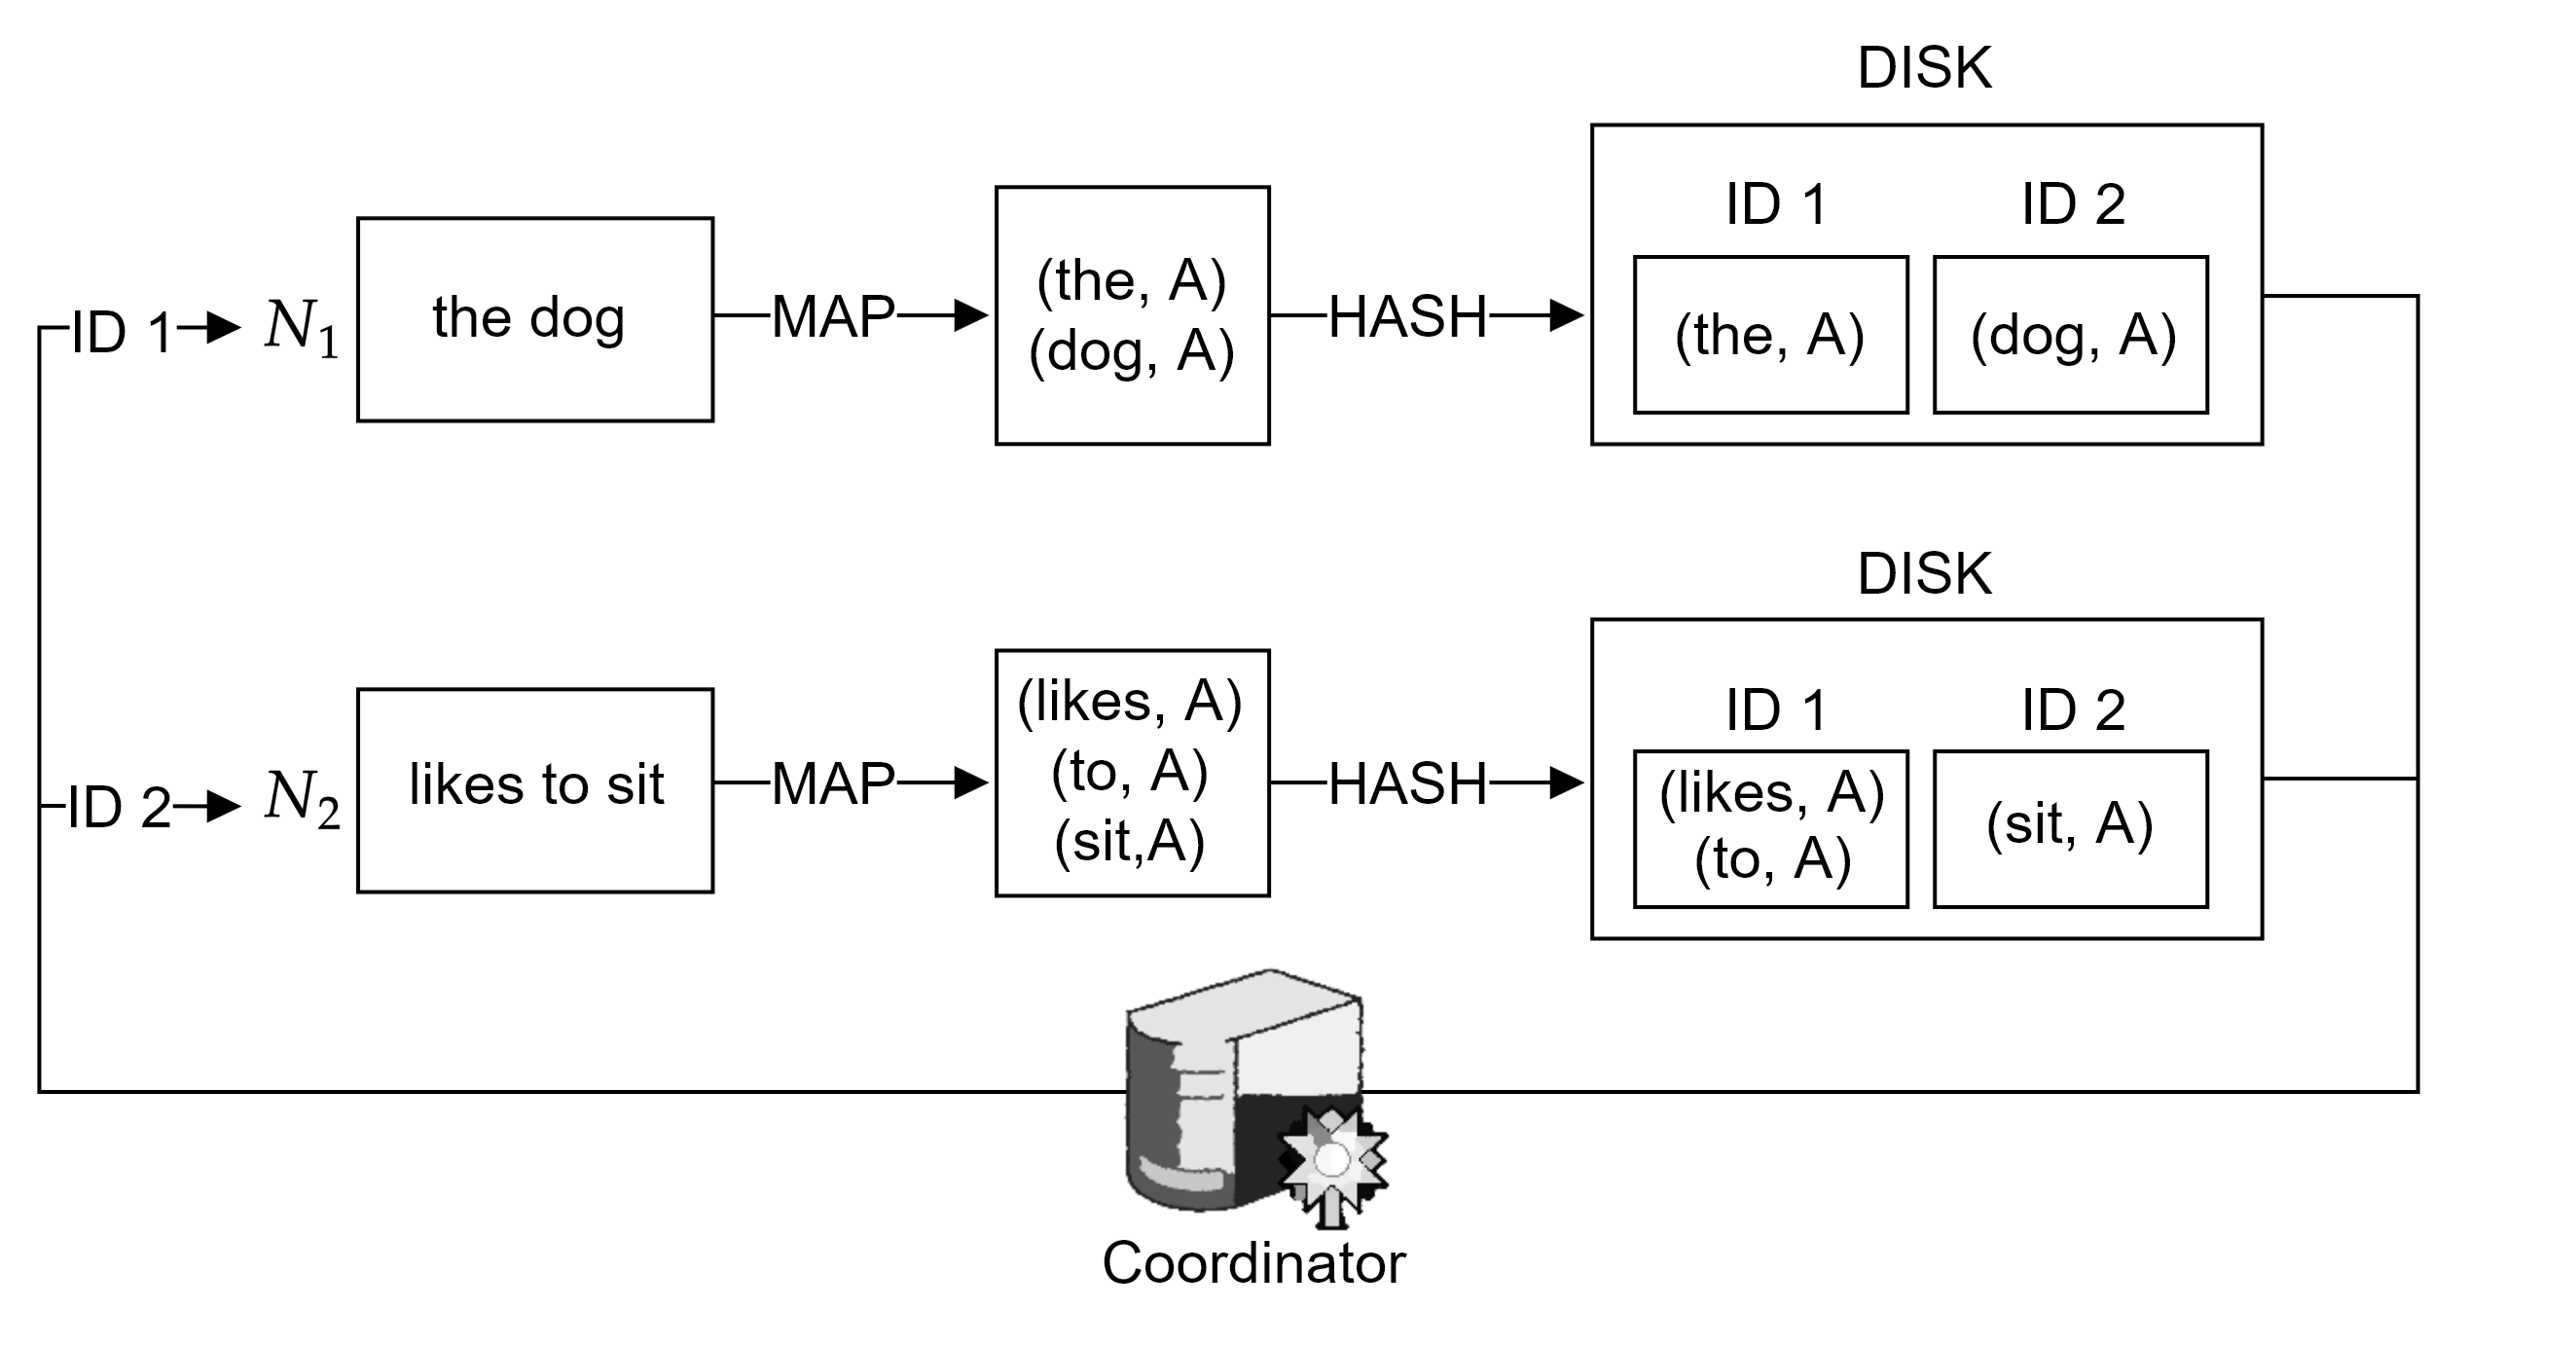
\includegraphics[width=\linewidth]{Sections/mapreduce/nwork.png}\\
\noindent
\rule{\linewidth}{0.4pt}\\

\hspace{-1.5em}
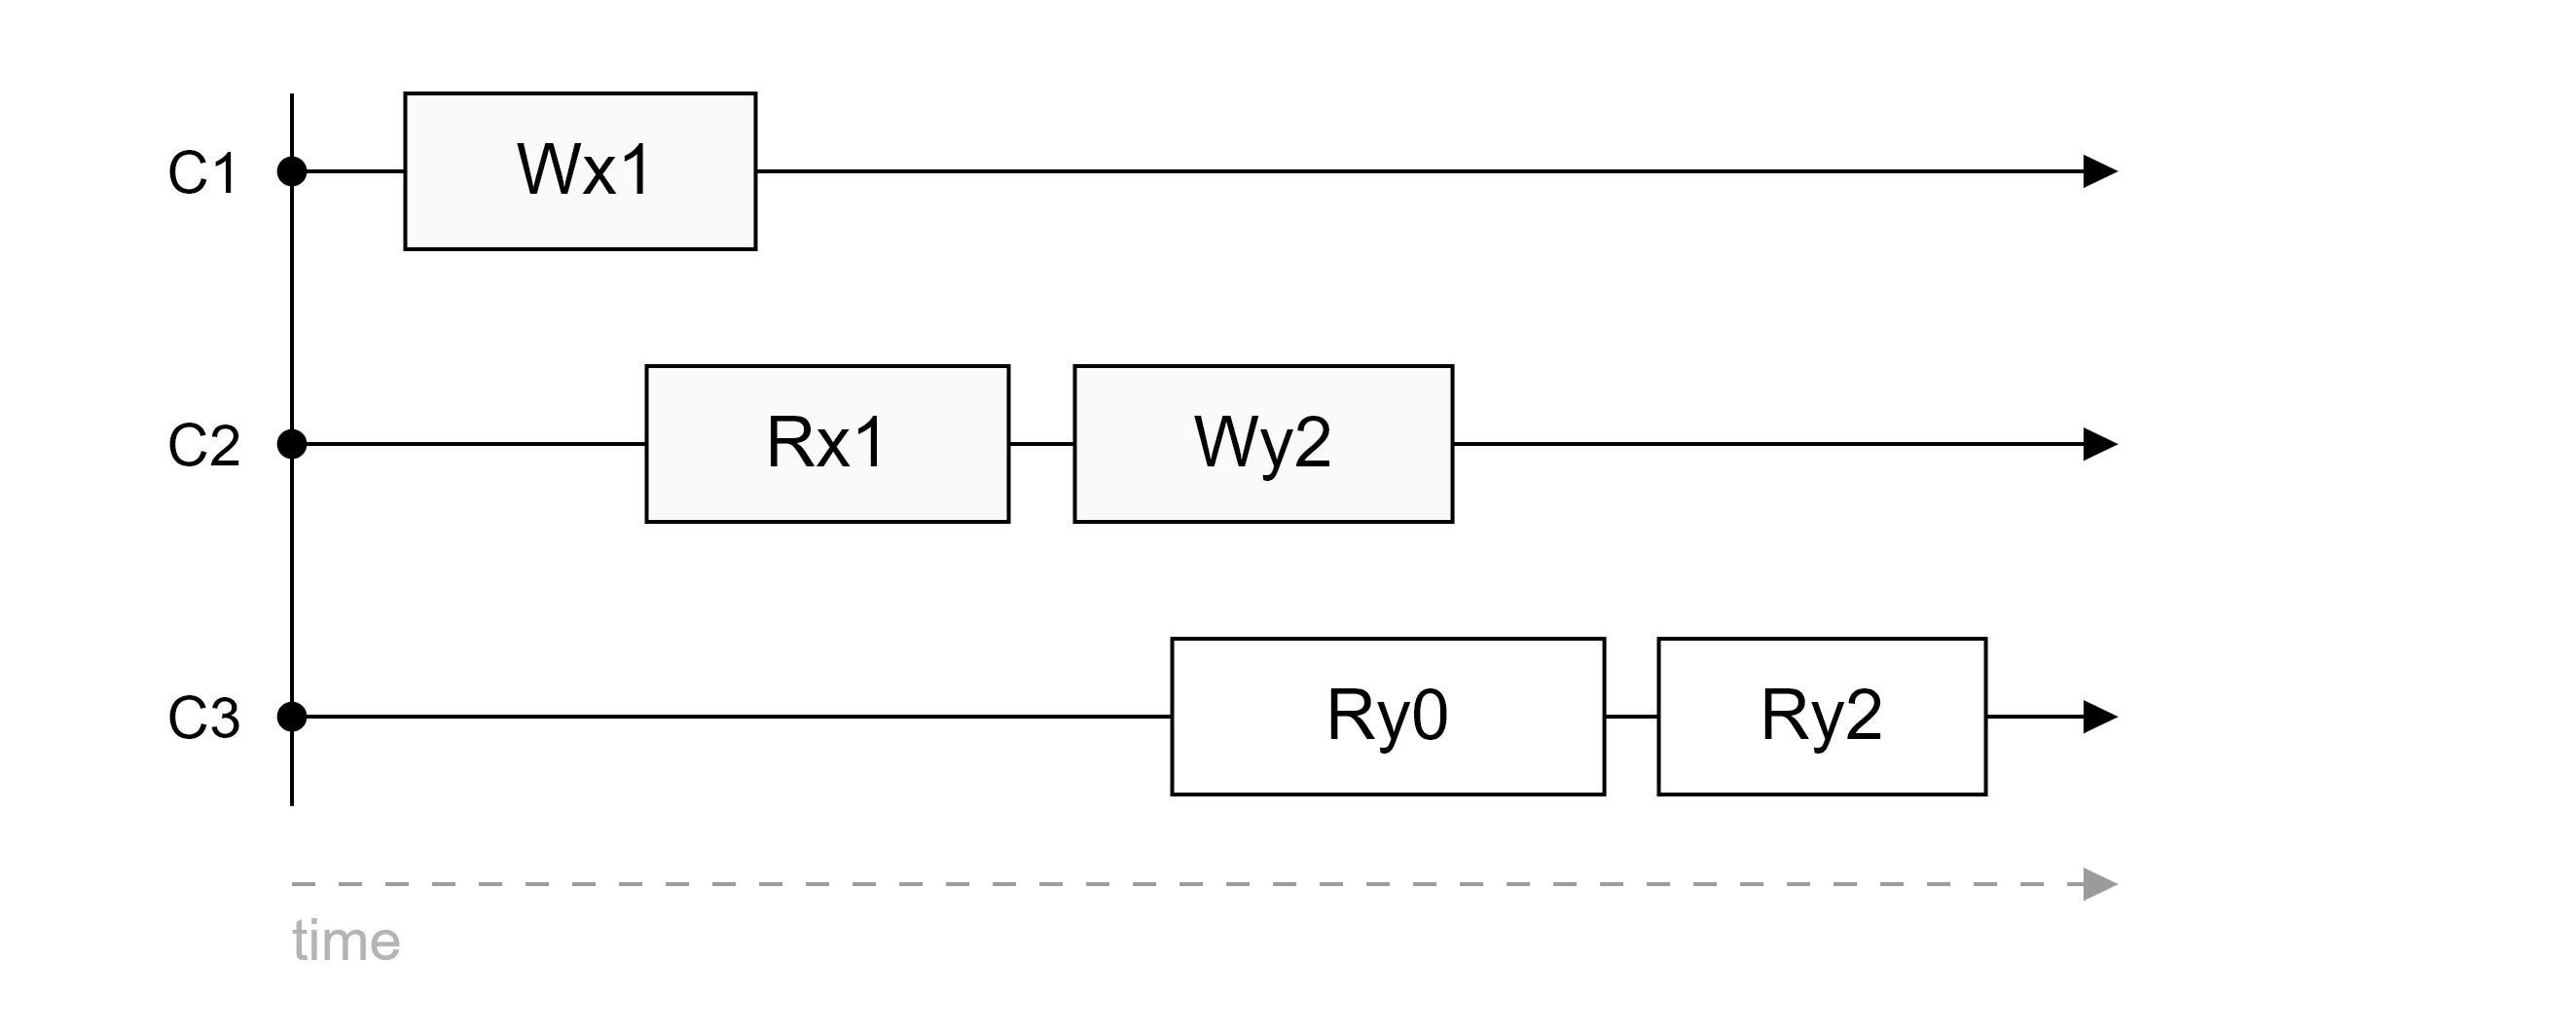
\includegraphics[width=\linewidth]{Sections/consist/test.png}\\
\noindent
\rule{\linewidth}{0.4pt}\\

\hspace{-1.5em}
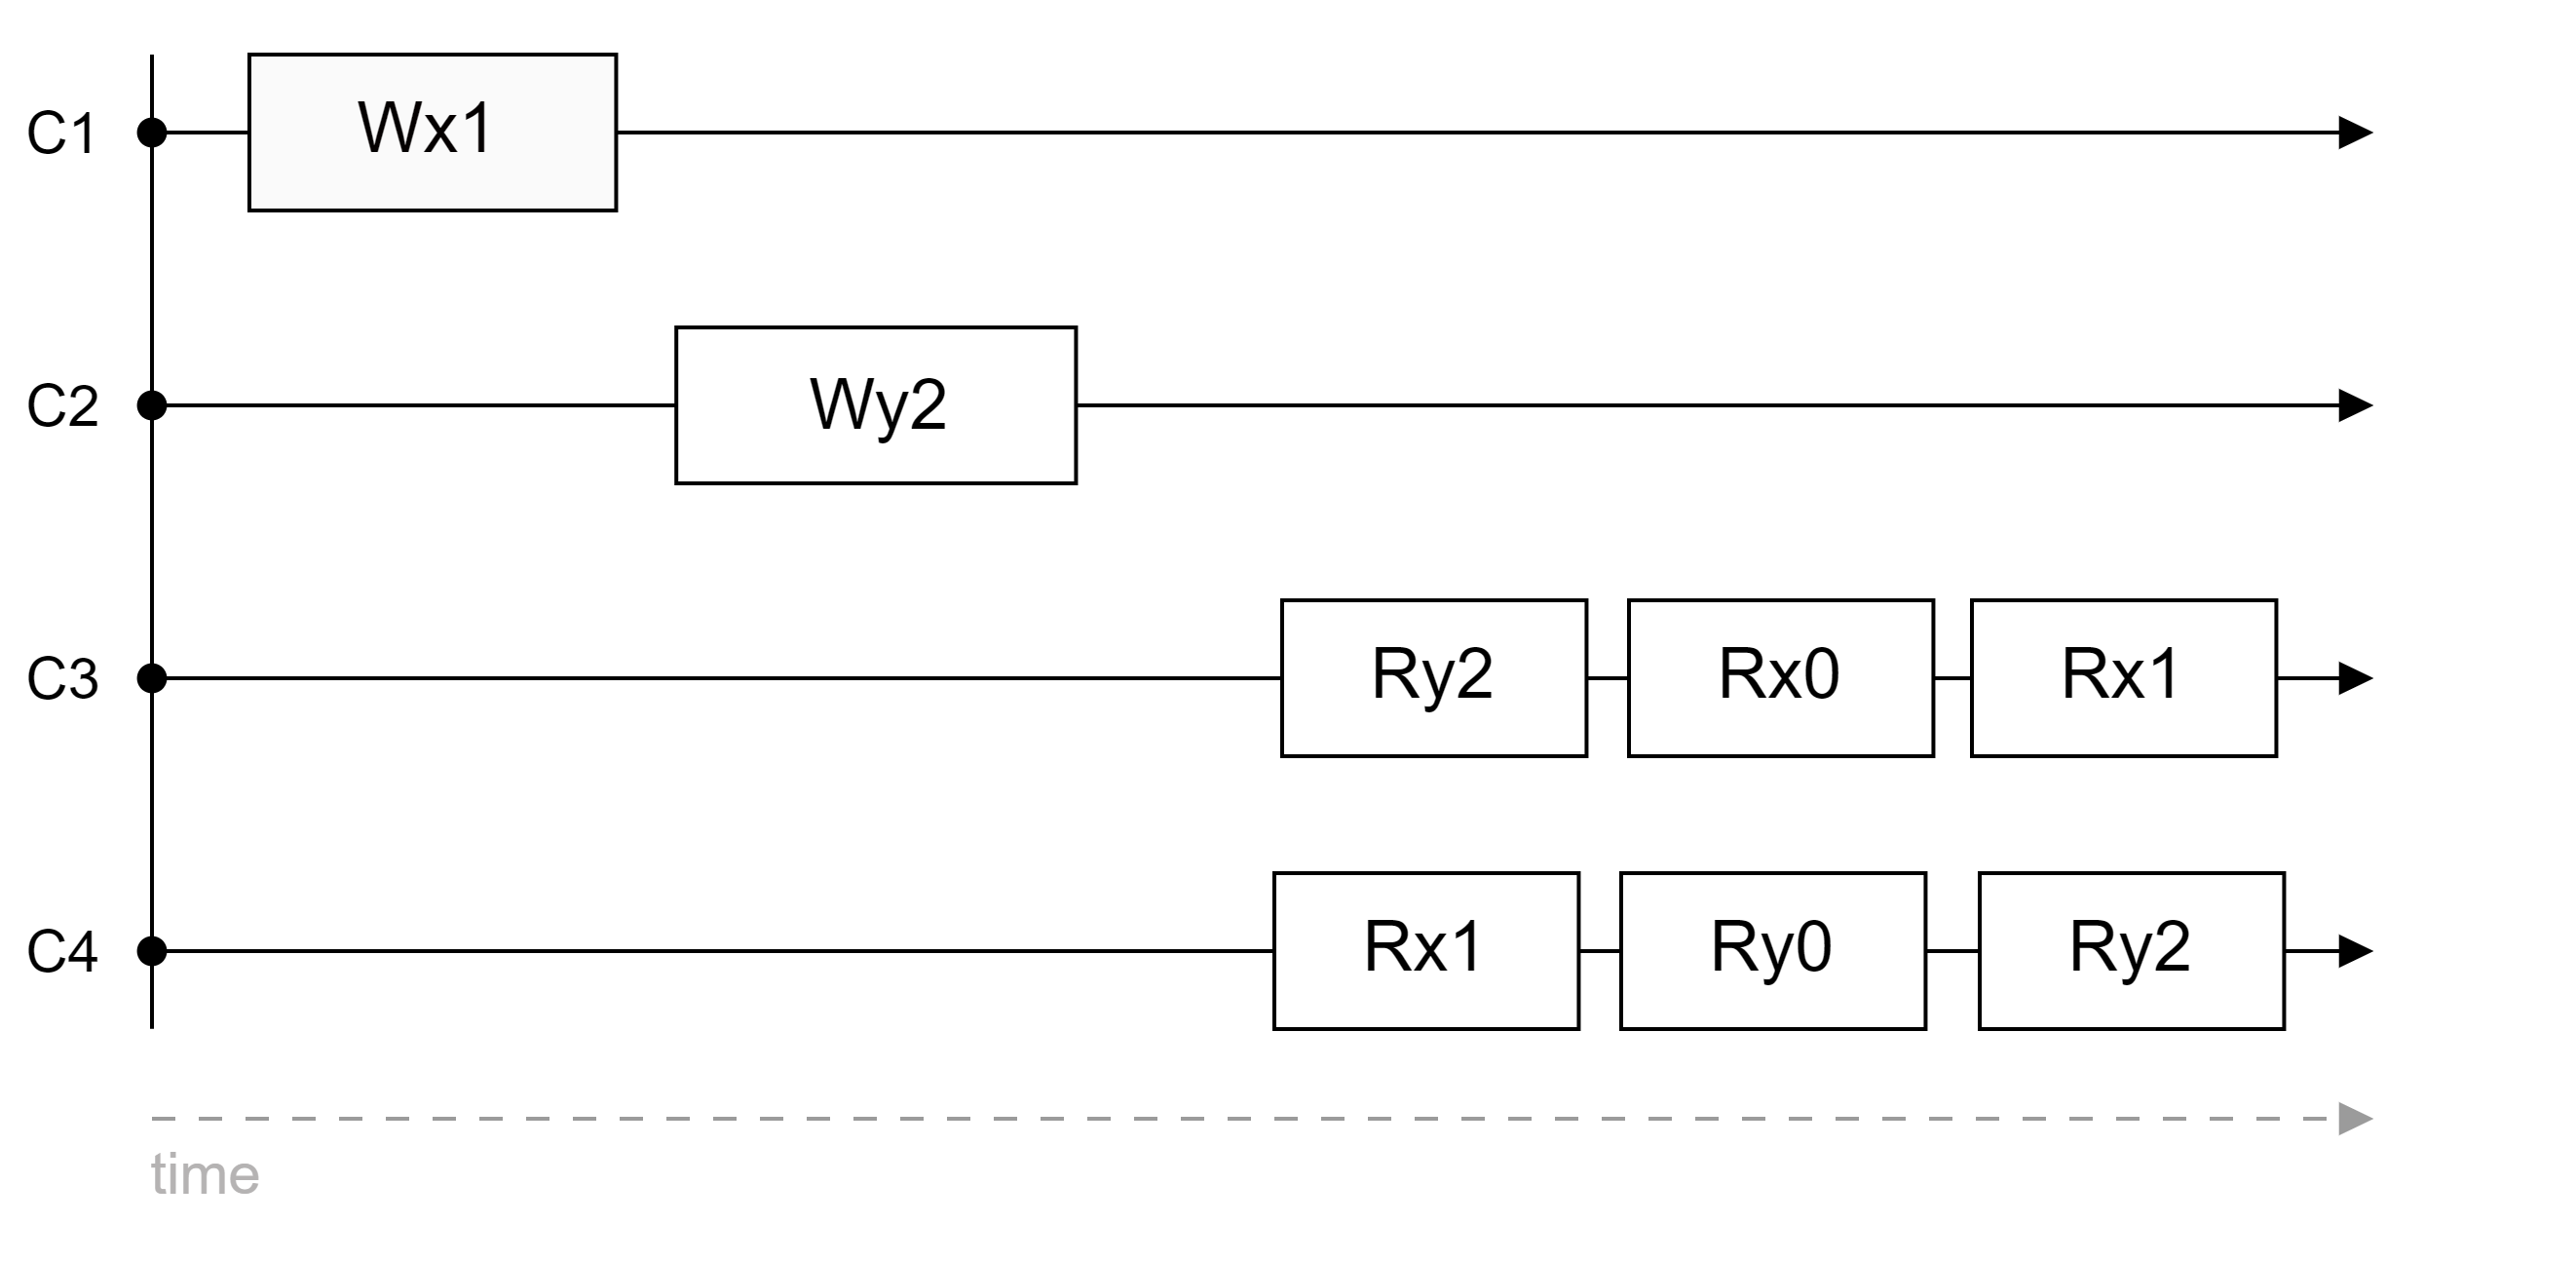
\includegraphics[width=\linewidth]{Sections/consist/event.png}\\
\noindent
\rule{\linewidth}{0.4pt}\\

\hspace{-1.5em}
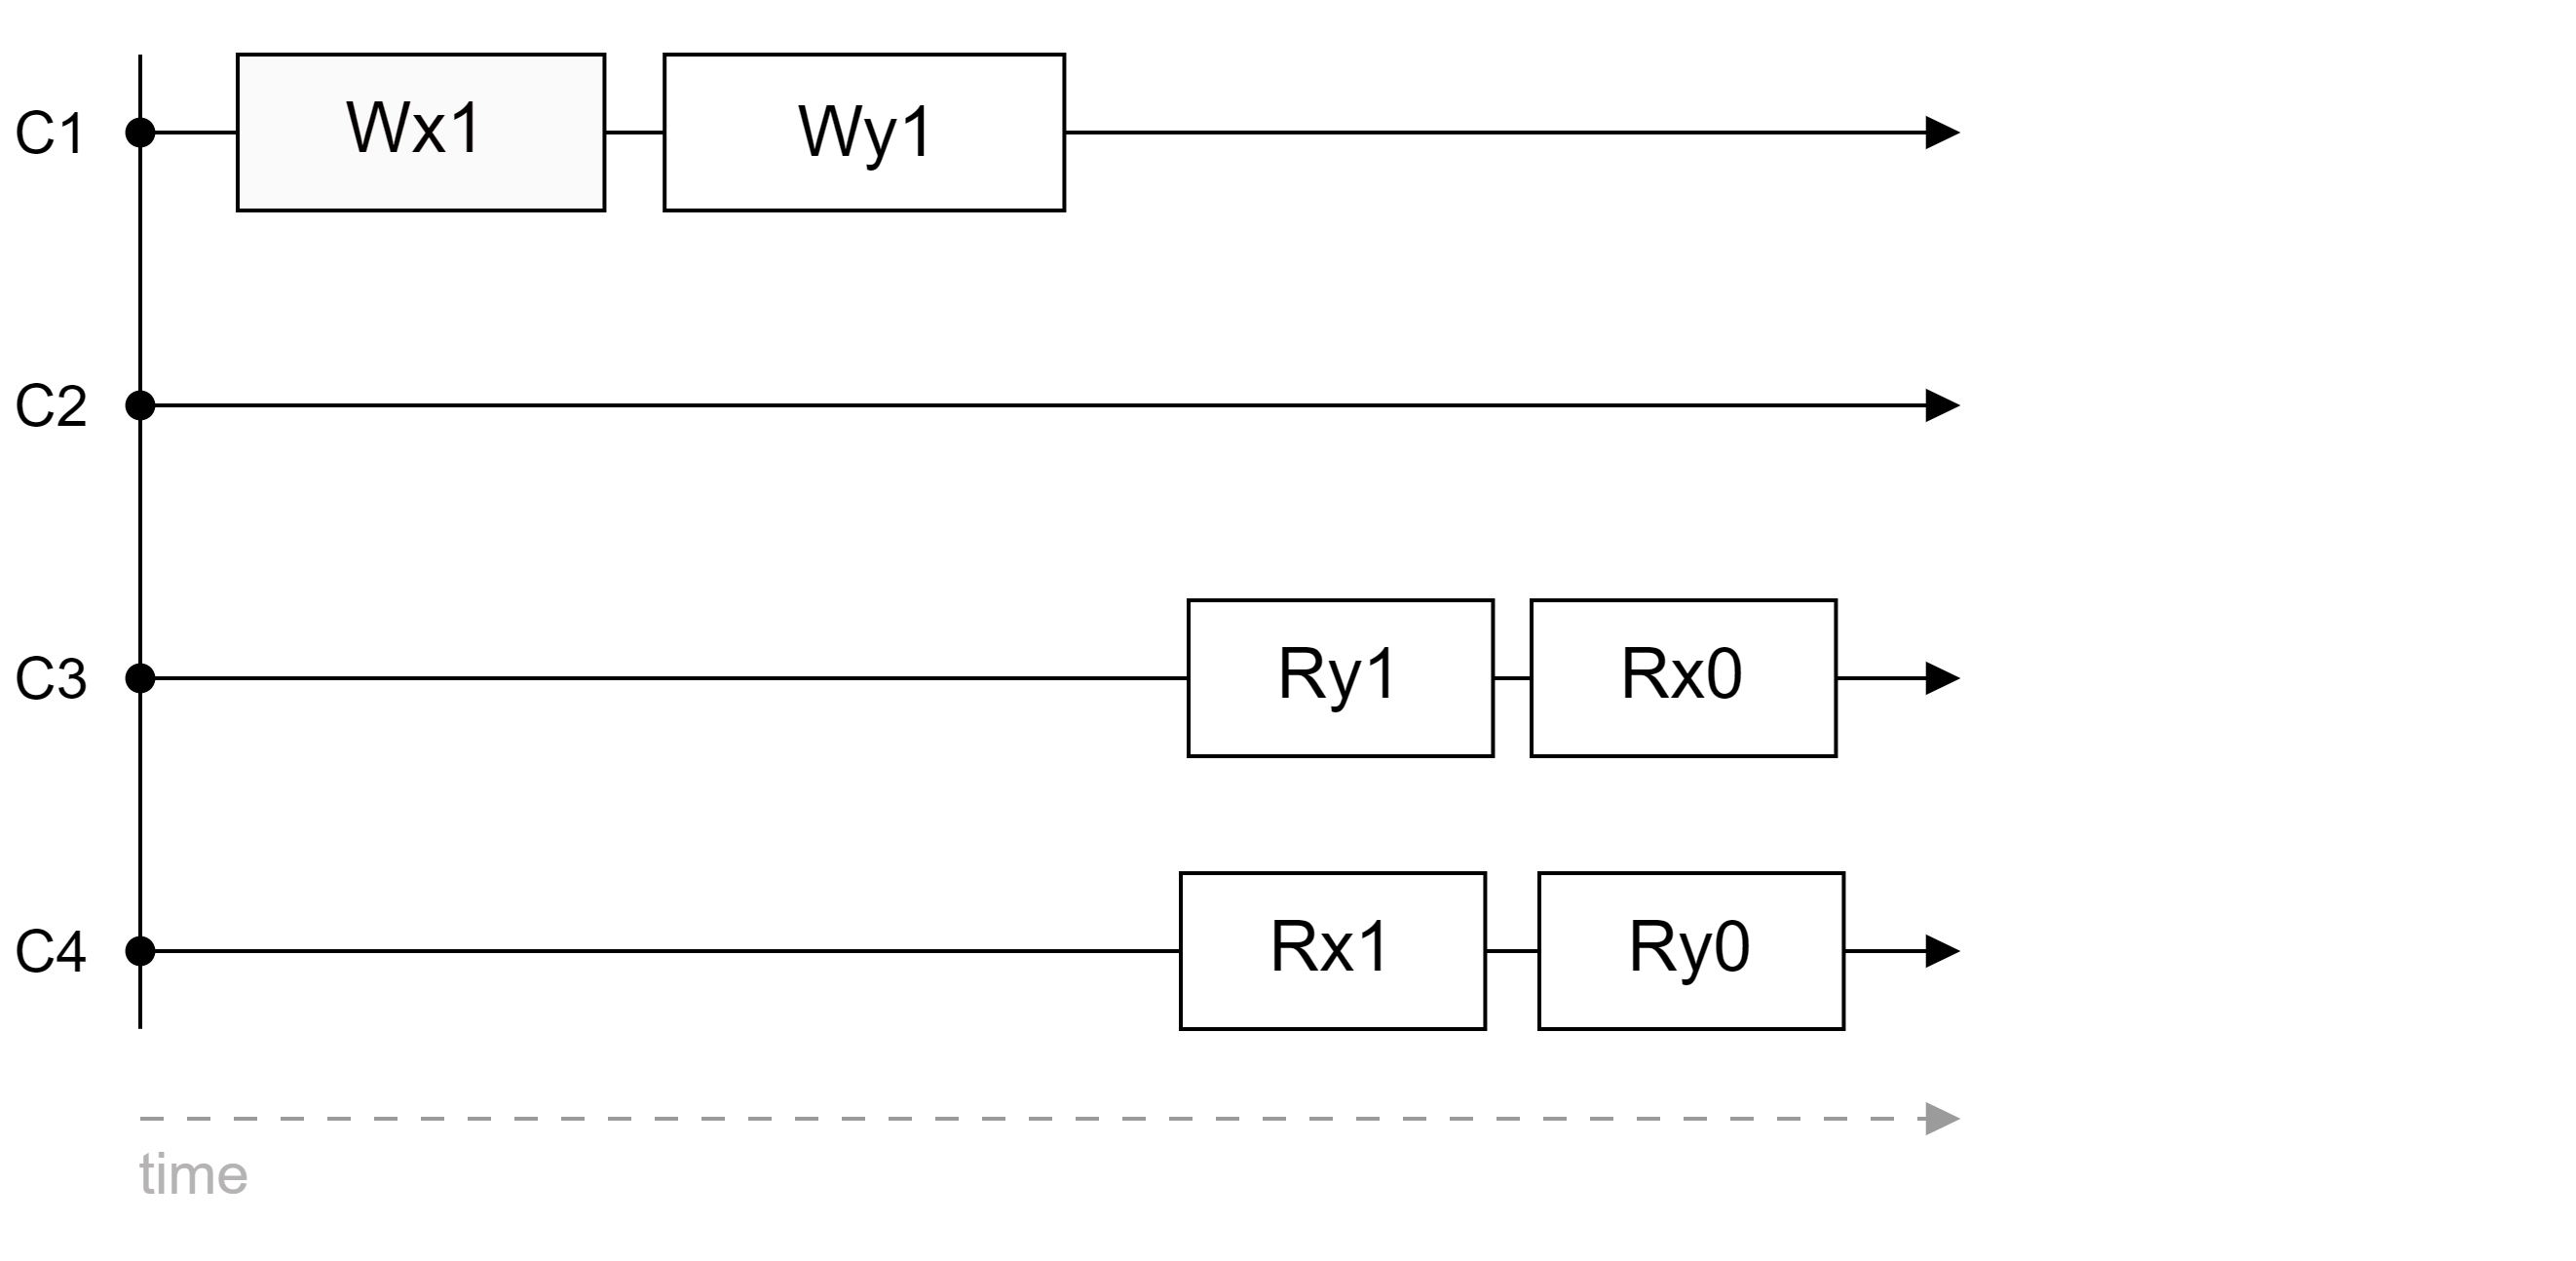
\includegraphics[width=\linewidth]{Sections/consist/seq3.png}\\




\end{multicols}


\newpage 

\begin{multicols}{2}

\noindent
---\textbf{Google File System (GFS)} (\ref{sec:gfs})---\textbf{Def (Wck):} Dist. file system, Scalable on cheap hardware, High availability on frequent failures (rep. need), High throughput of seq. reads and append-only writes.
Files are split into 64MB chunks, given a 64 bit ID chunk handle. Chunks must be replicated $N$ times (Typically $N=3$). There is 
one TC, the master, which manages the file$\to$chunk mappings and access control information.
The client queries the master with (file name, chunk index), and receives the replica location.
It caches this information to speak with the server directly. Clients may directly read from any chunk server (stale reads allowed).
For writes, the client sends data to the closest replica, which then forwards it to the next closest replica.
After all is done, the client orders the primary replica (picked by the master with a timed lease) to commit the data. The primary
eagerly commits their own state and replies success, while the others lazily commit their state. The 
master will periodically check for stale chunks in case of failures (garbage collection through heartbeats). 
There are also background master replicas (shadows) that locally replay the master state in case of failure.
The master has checkpoints, which are snapshots that truncates the log. Shadows also serve as read-only replicas to reduce load on the master.
Shadows exhibit eventual consistency, slightly lagging behind the master.
There is non-atomicity and non-serializability across chunks, but there is within a single chunk, due to the order of
accepted writes from a primary on any given chunk. If a write is rejected as per full chunk, the client must refresh (find the new chunk server) from the master.
Having a single master simplifies the design of the
system.---\textbf{Dynamo: Key-Value store} (\ref{sec:dynamo})---\textbf{Def (Wck):} Always writeable (high availability), scalable, decentralized, low-latency performance (SLA: Service Level Agreement of 300ms on 99.9\% of requests),
Eventual consistency. Utilizes consistent hashing on 128-bit ordered list of $N$ virtual nodes. Writes:
client sends put(key, value), which is hashed to $N_j$, which serves as the coordinator/owner of the key. Such coordinator propagates in parallel to the next $N-1$ healthy nodes (preferred list). After 
$W$ servers respond, the coordinator sends a success to the client. Reads: client sends get(key), which is hashed to $N_j$, who waits for $R$ responses from the preferred list. 
Quorum Condition: $W+R > N$, ensures sufficient overlap, mitigating stale reads. Failure:
If $k$ hashes to $A$'s segment, we retry the next healthy node. We hint (notify) the next node $B$ that $A$ is down. $B$ then stands in as 
the coordinator, with the addition of hinting $A$ to the cluster (Sloppy Quorum). During runtime, all $N$ nodes gossip with each other, sending heartbeats at random. During this phase,
if $A$ recovers, a random server $C$ may notice this, and preform a hinted-handoff, passing along the operations $A$ missed. Diverging data is 
resolved via a versioning vector clock for each object (key, value), where each cell is a node, and the value is a monotonically increasing counter of its participation.
During reads, the coordinator attempts to resolve the vector clock, if it can't, it returns all versions to the client. The client must decide how to merge the data (often unioning them in case of two carts).
Then sends the merged data back as a put operation. In the background, nodes will try to resolve stale data via merkle trees (hash trees). Merkle trees, first hash a range of keys (leaves), then combines two 
hashes into a parent (intermediate nodes), until they reach the root node (summarizes the entire tree). Nodes use this to efficiently find divergent data. GFS.

\noindent
\rule{\linewidth}{0.4pt}\\

\hspace{-1.5em}
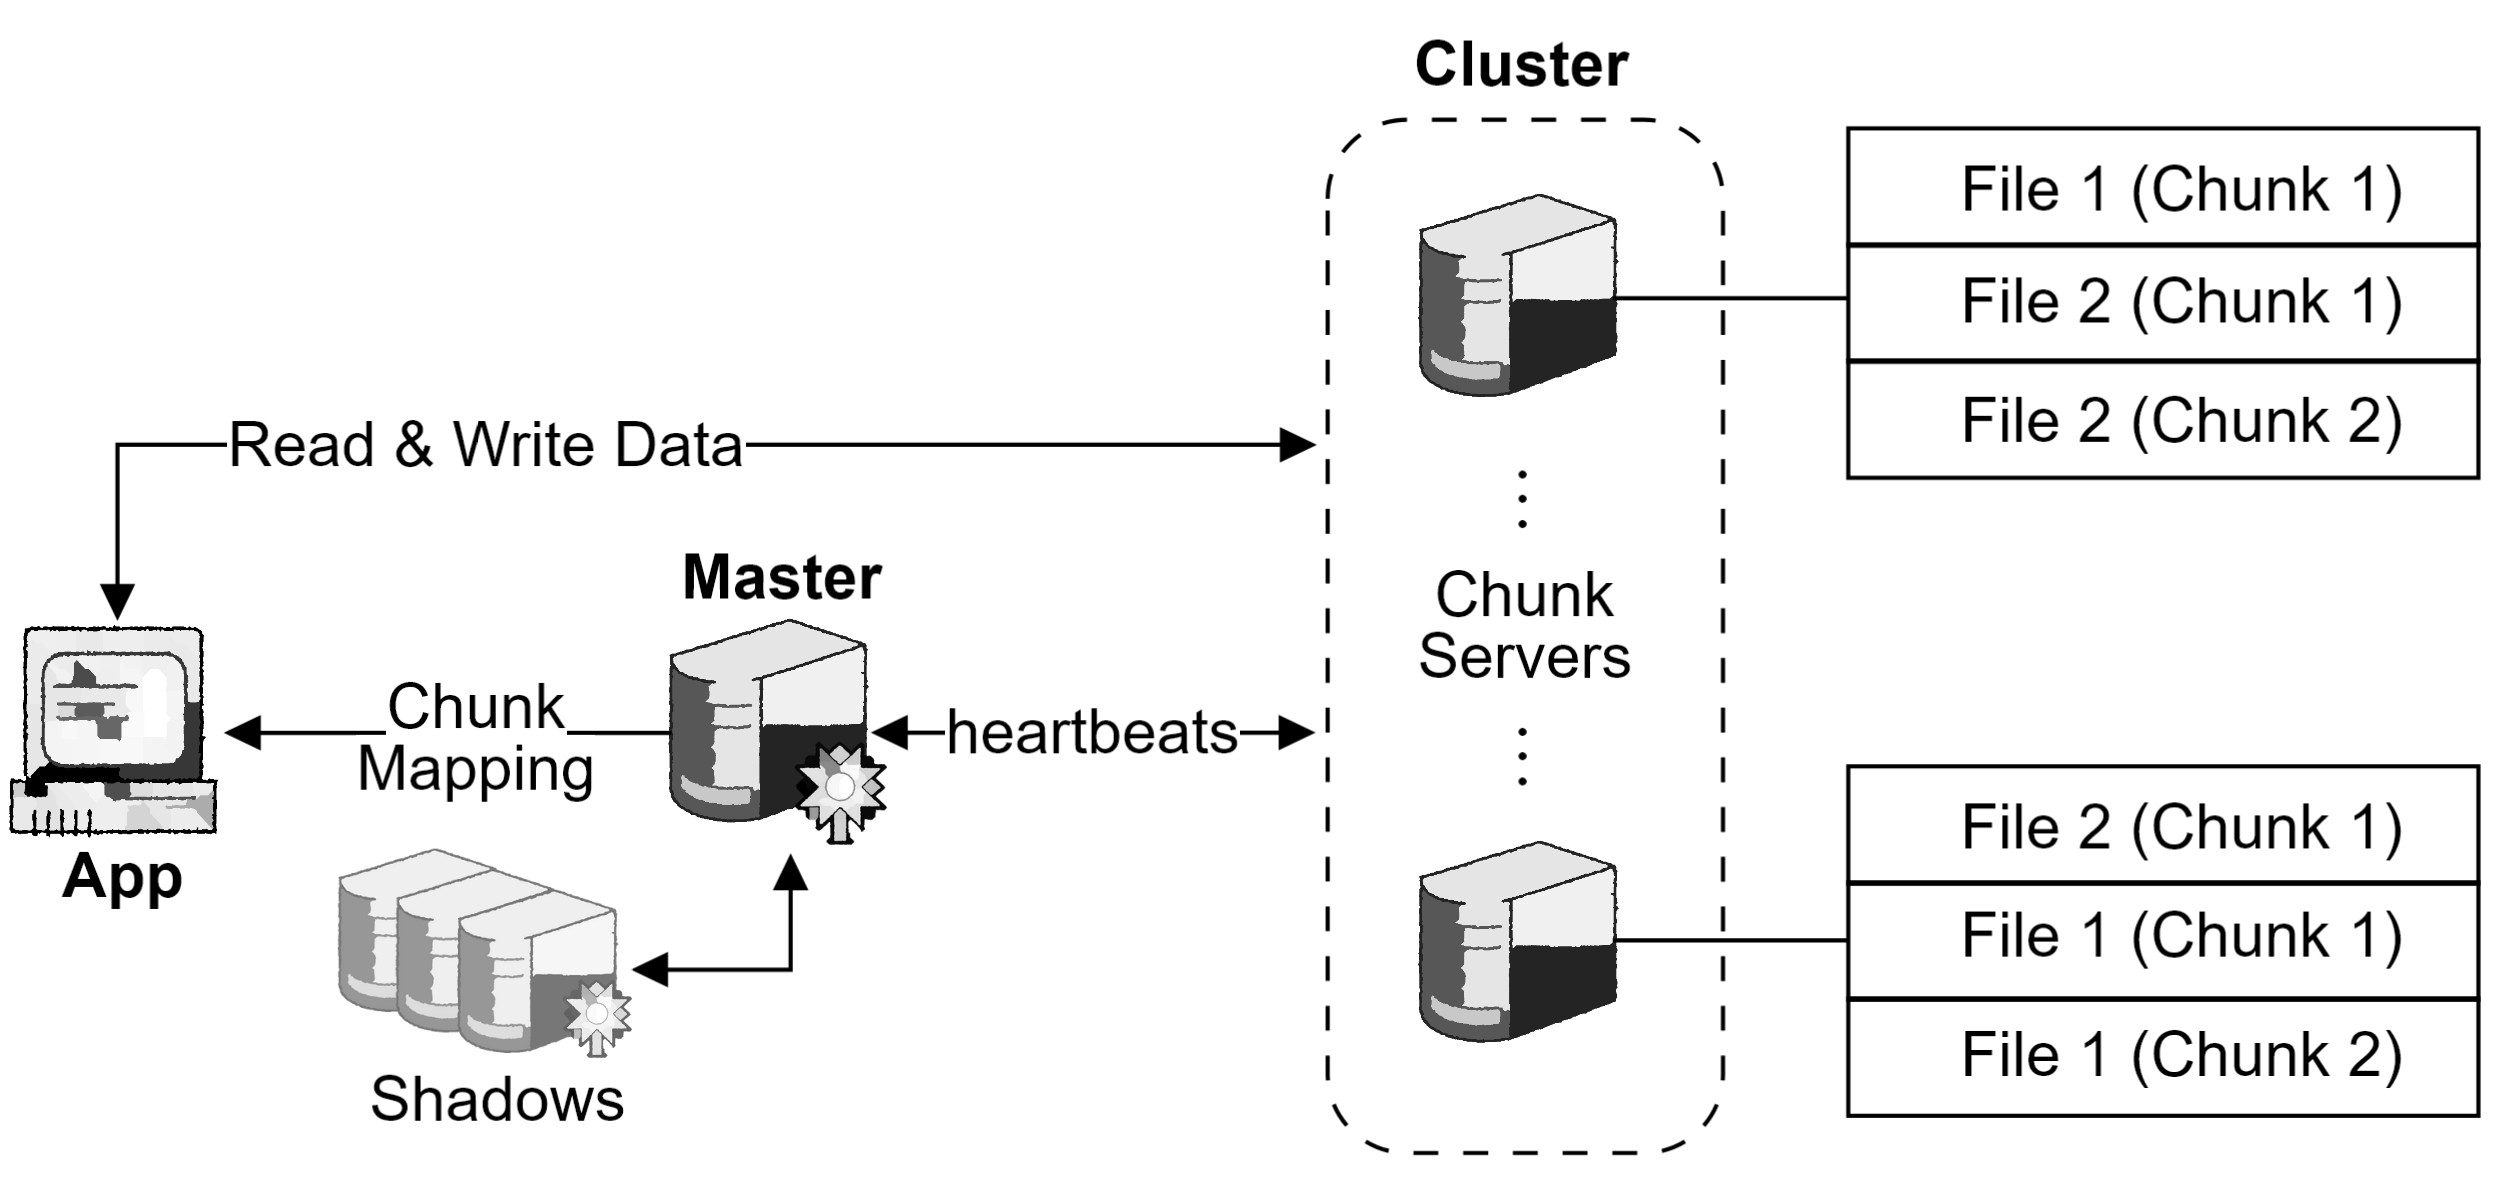
\includegraphics[width=\linewidth]{Sections/gfs/high.png}\\


\end{multicols}


\begin{multicols}{2}

\noindent
---\textbf{Spanner} (\ref{sec:spanner})---\textbf{Def (Str):} A globally distributed database, linearizeble reads and writes across shards (globaly agreed timestamp), High availability, low-latency, lock-free read-only transactions, strict serializability, with atomic transactions.
Utilizes Multi-Version Concurrency Control (MVCC): Each write transaction assigned a uniquely increasing timestamp with every key-value pair.
Safe Time Rule: Before transaction $T$ reads key $k$, it must see a timestamp greater than the last write to $k$ (if any).
Atomic clocks are used to mitigate clock drift, and are synchronized via GPS satellites. The TrueTime API, provides a \texttt{TT.now()}, which returns  a $[t_{earliest}, t_{latest}]$ interval, where the real time must be between the two (inclusive).
The difference of the two intervals is the uncertainty $\delta$, which is the time it must wait before reads or writes can be performed.
The protocol uses paxos (consensus model like raft) to ensure fault-tolerance and availability of replicas. Read-write Transactions:
two-phase locking (2PL) and two-phase commit (2PC) are used to ensure isolation and atomicity respectively. The first phase acquires locks on needed keys and reads the values, then 2PC commences with one of the shard paxos leaders as the TC.
After the commit, the locks are released.---\textbf{TLA$+$} (\ref{sec:tla})---is a high-level specification language based on temporal logic that lets you model distributed
algorithms, exhaustively explore all possible states, and prove safety and liveness properties. While
it excels at uncovering subtle bugs and proving correctness, TLA$+$ specifications do not translate
directly into production code—implementing a verified design remains a substantial engineering
effort.\\
CHash. Caus\&Seq. HintOff. DynCliRec. Merkle.

\noindent
\rule{\linewidth}{0.4pt}\\
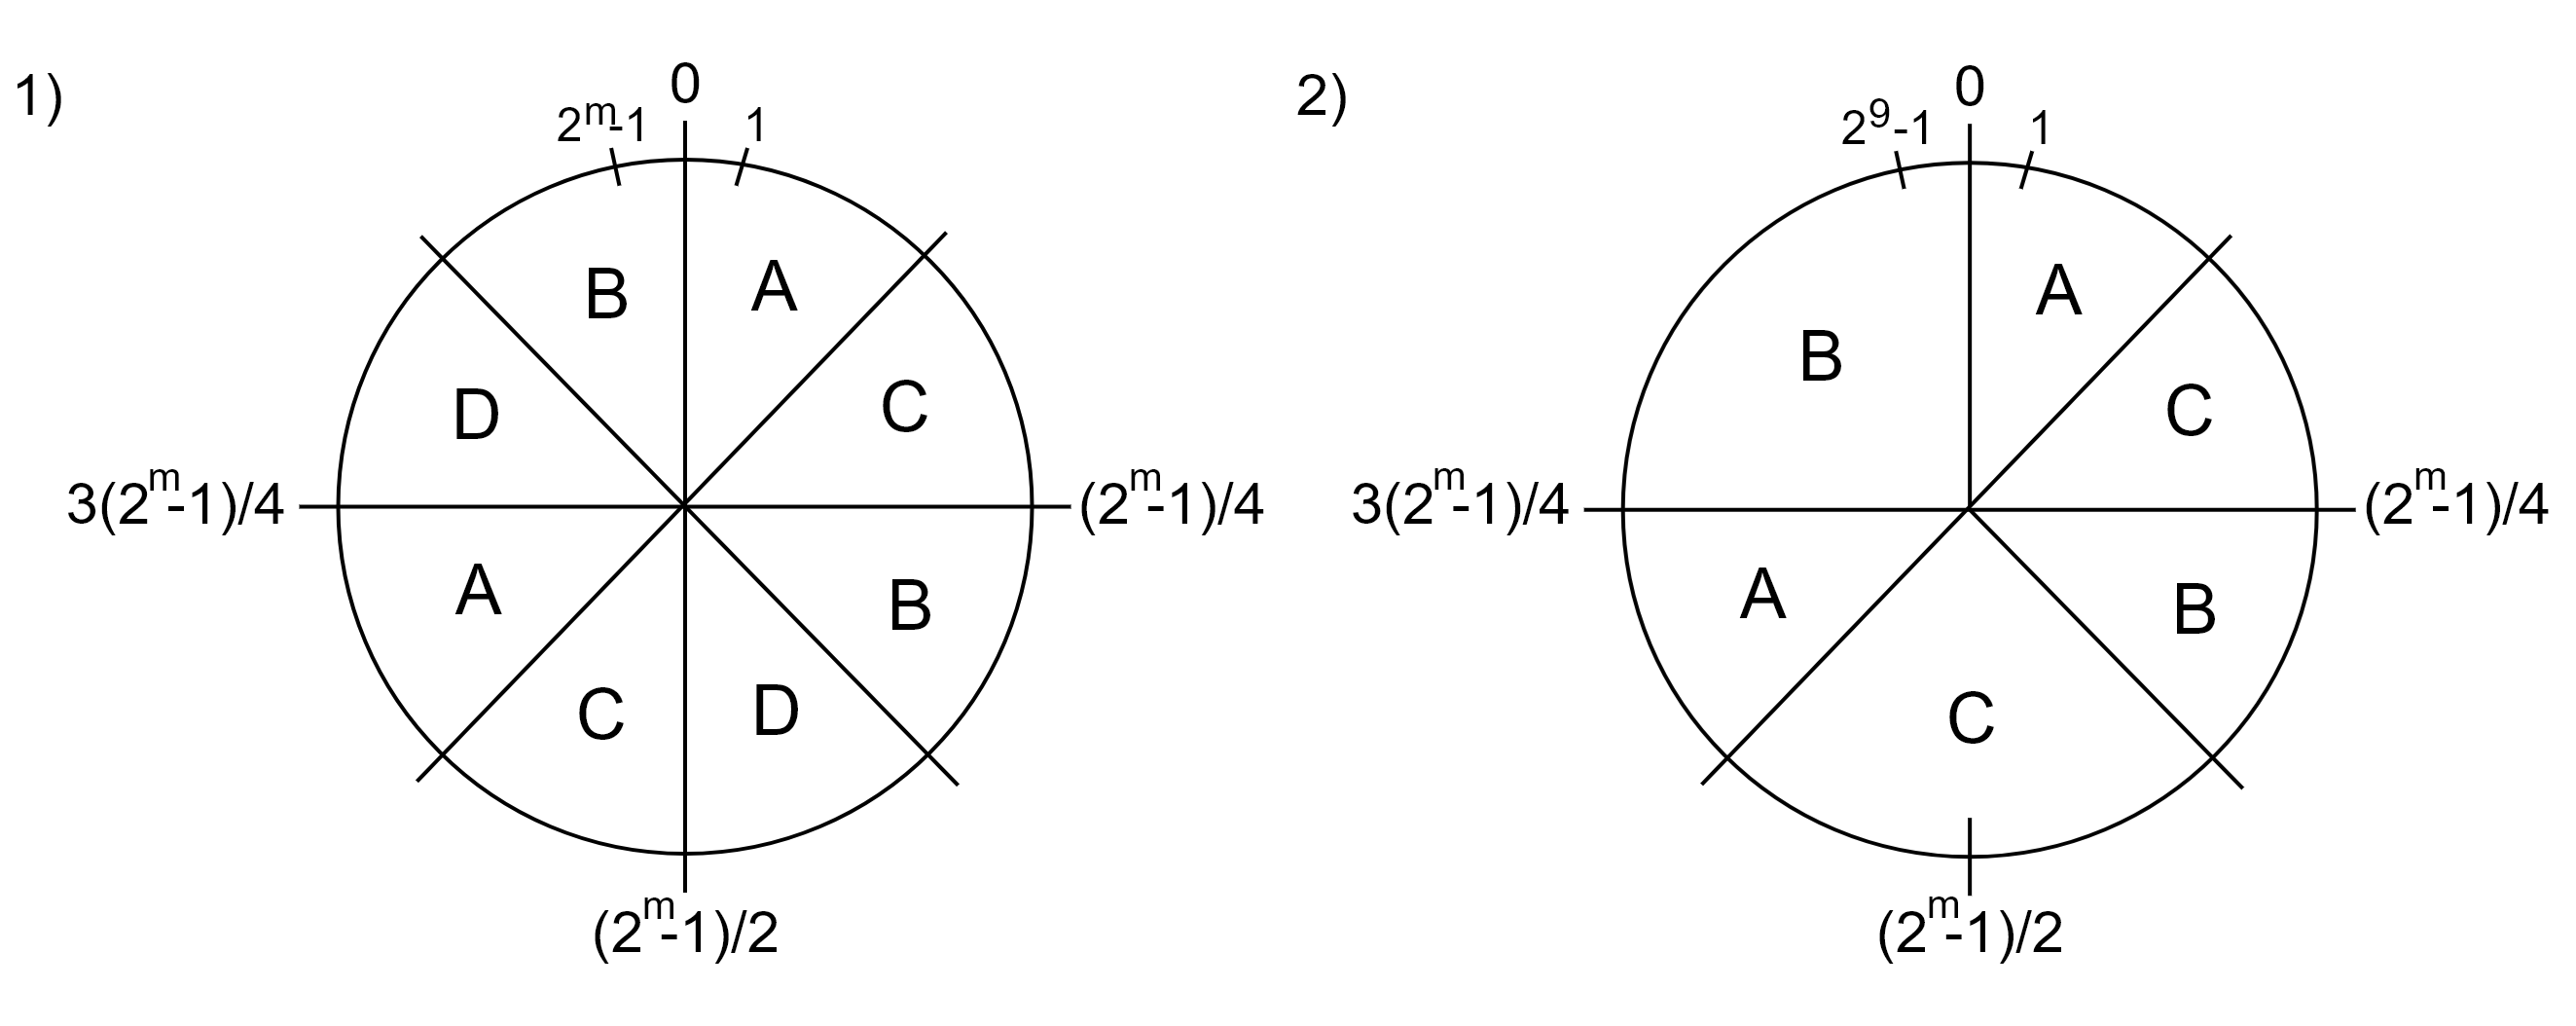
\includegraphics[width=\linewidth]{Sections/shard/ring_2.png}\\

\vspace{-2em}

\noindent
\rule{\linewidth}{0.4pt}\\
\hspace{-1.5em}
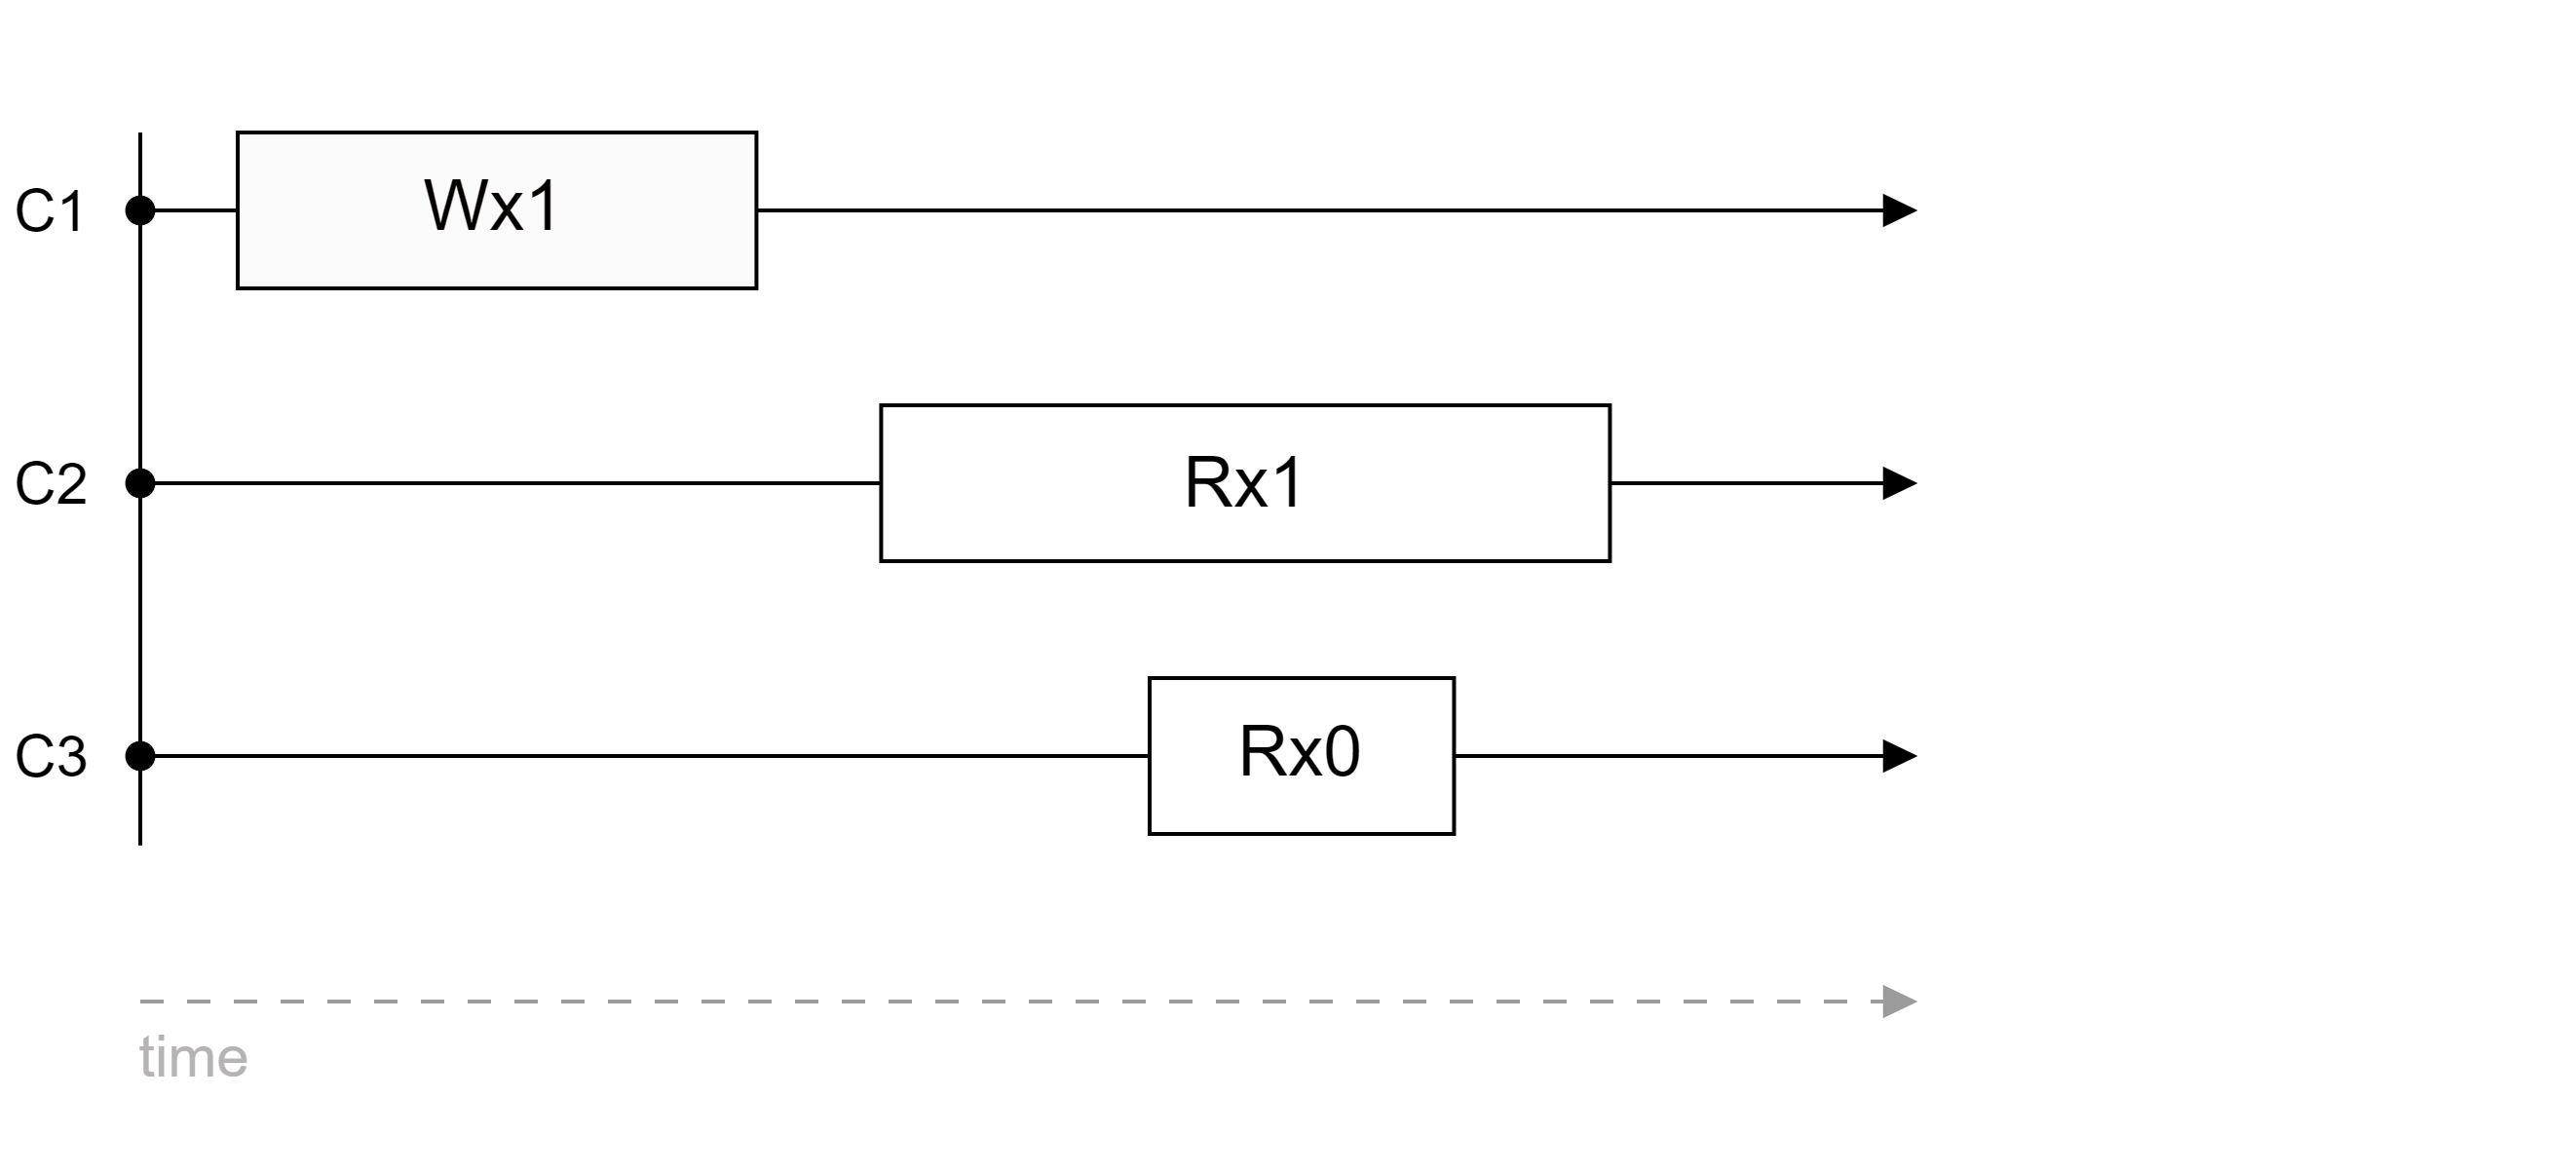
\includegraphics[width=\linewidth]{Sections/consist/cas1.png}\\

\vspace{-3em}
\hspace{-2.5em}
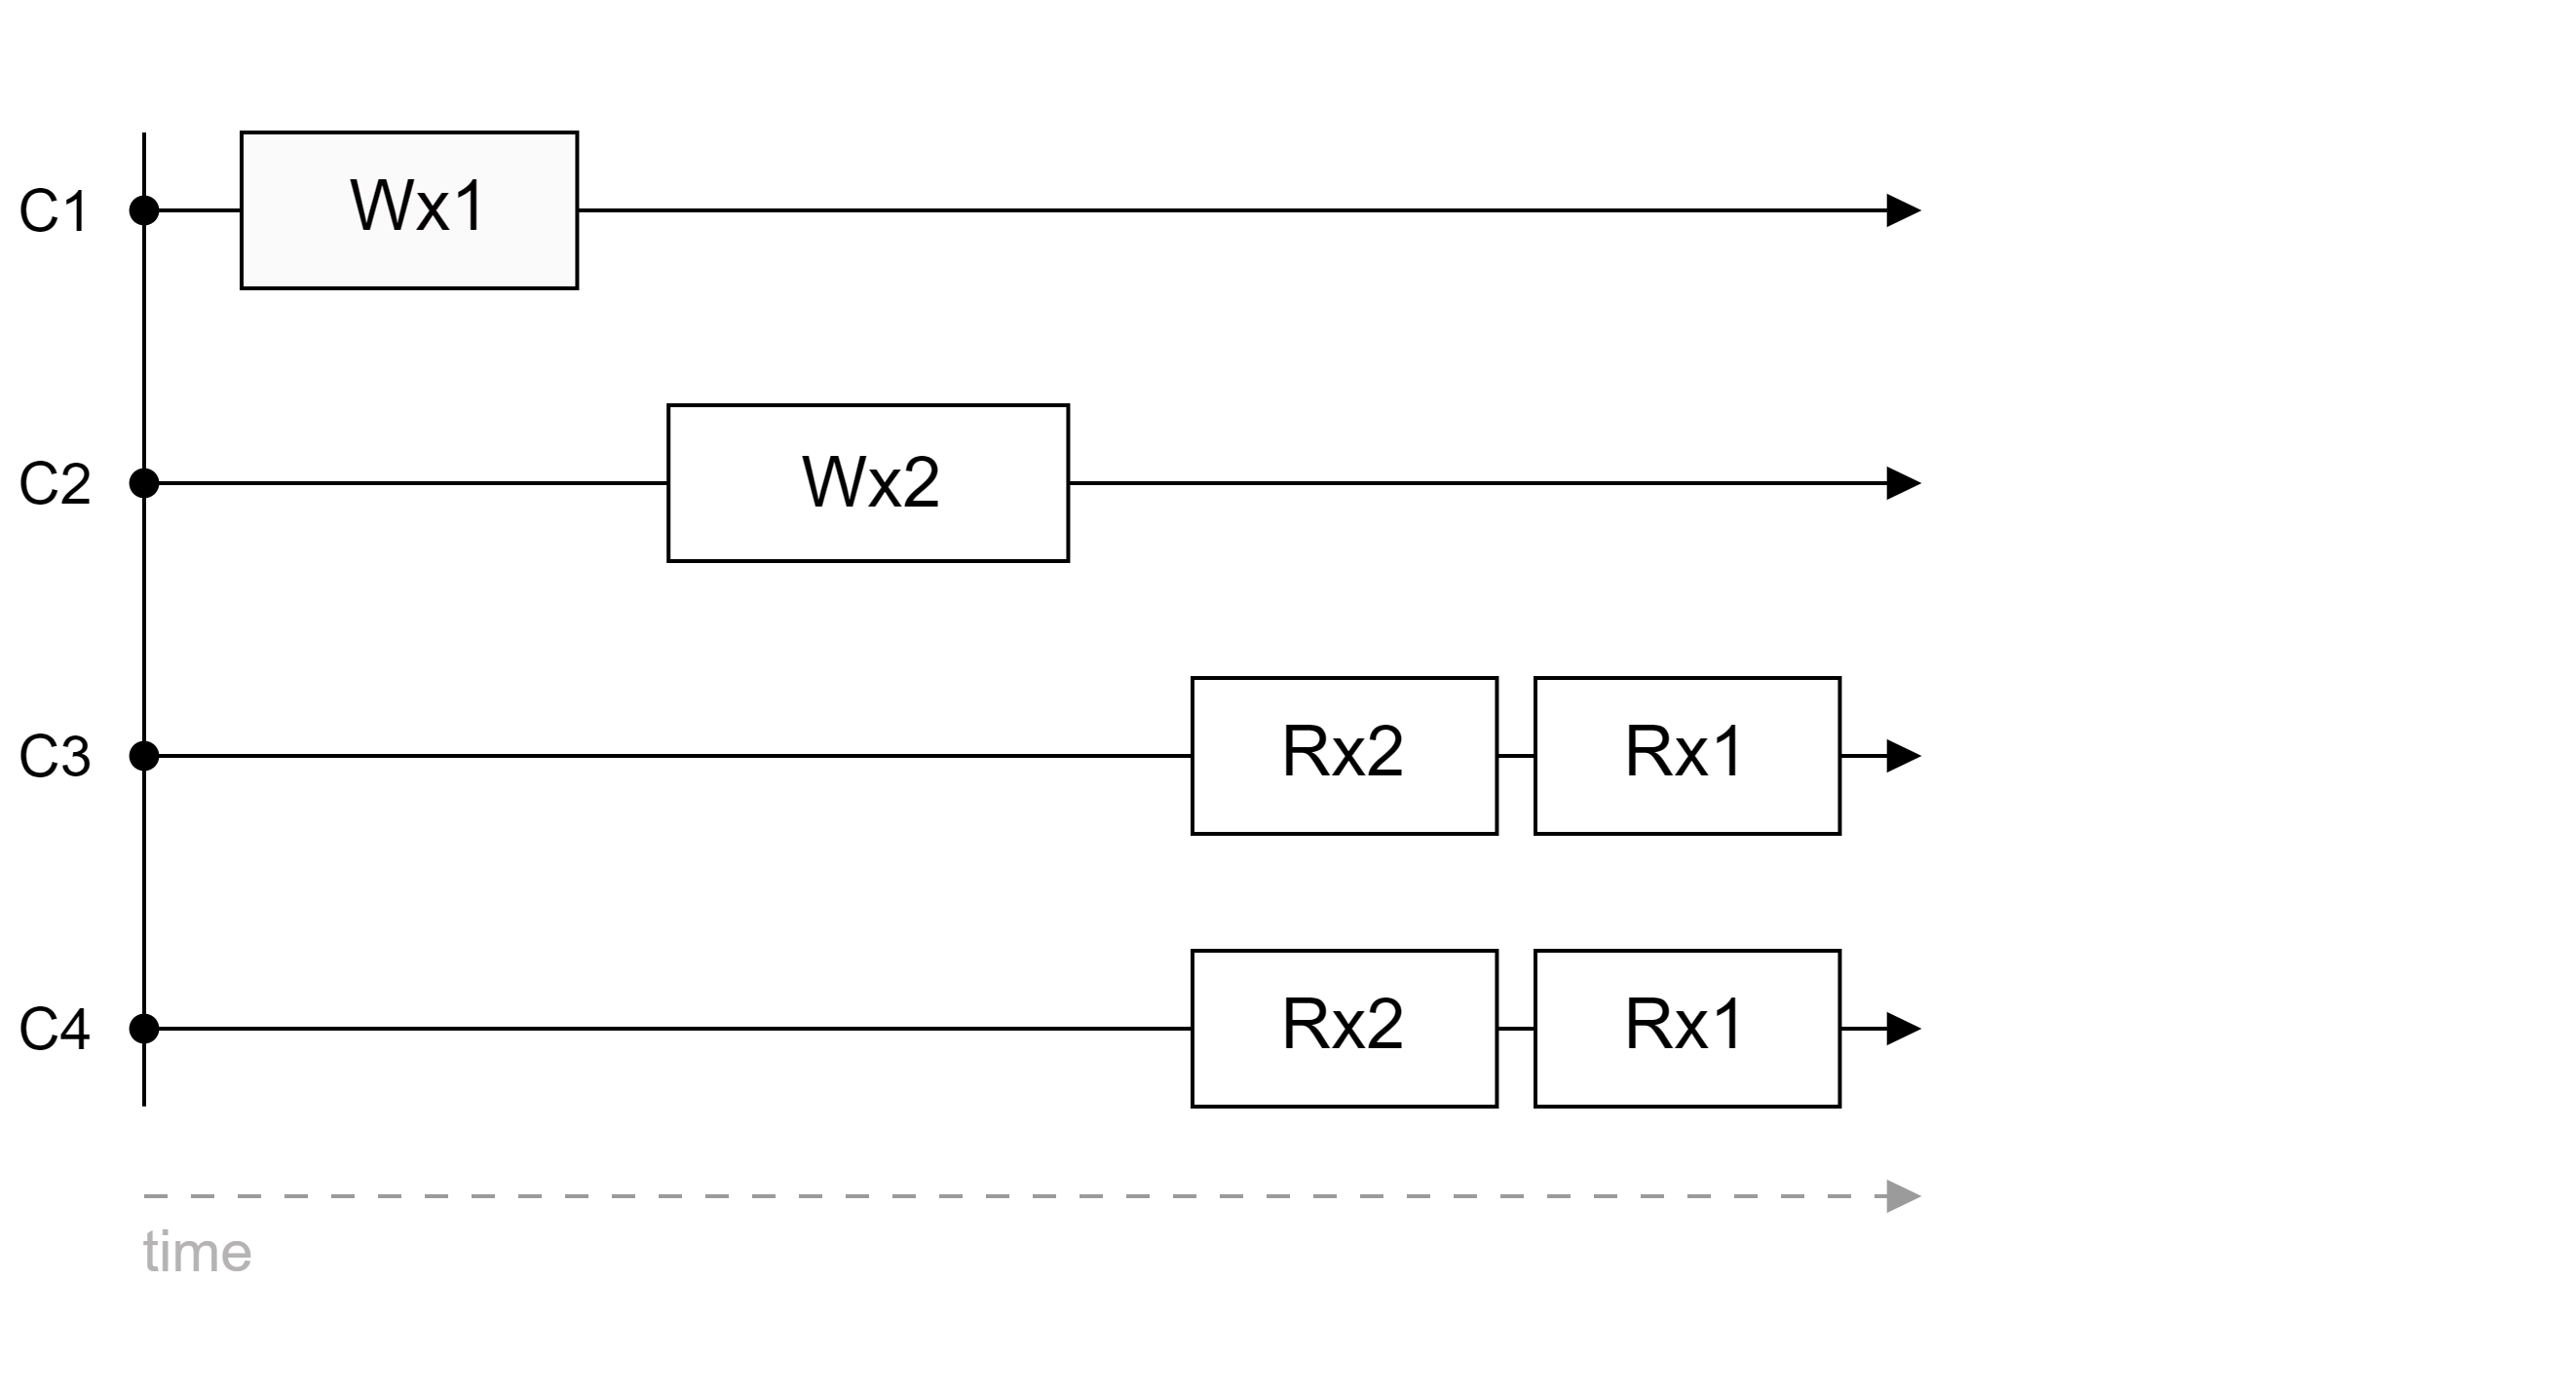
\includegraphics[width=\linewidth]{Sections/consist/seq1.png}\\
\noindent
\rule{\linewidth}{0.4pt}\\

\hspace{-1.5em}
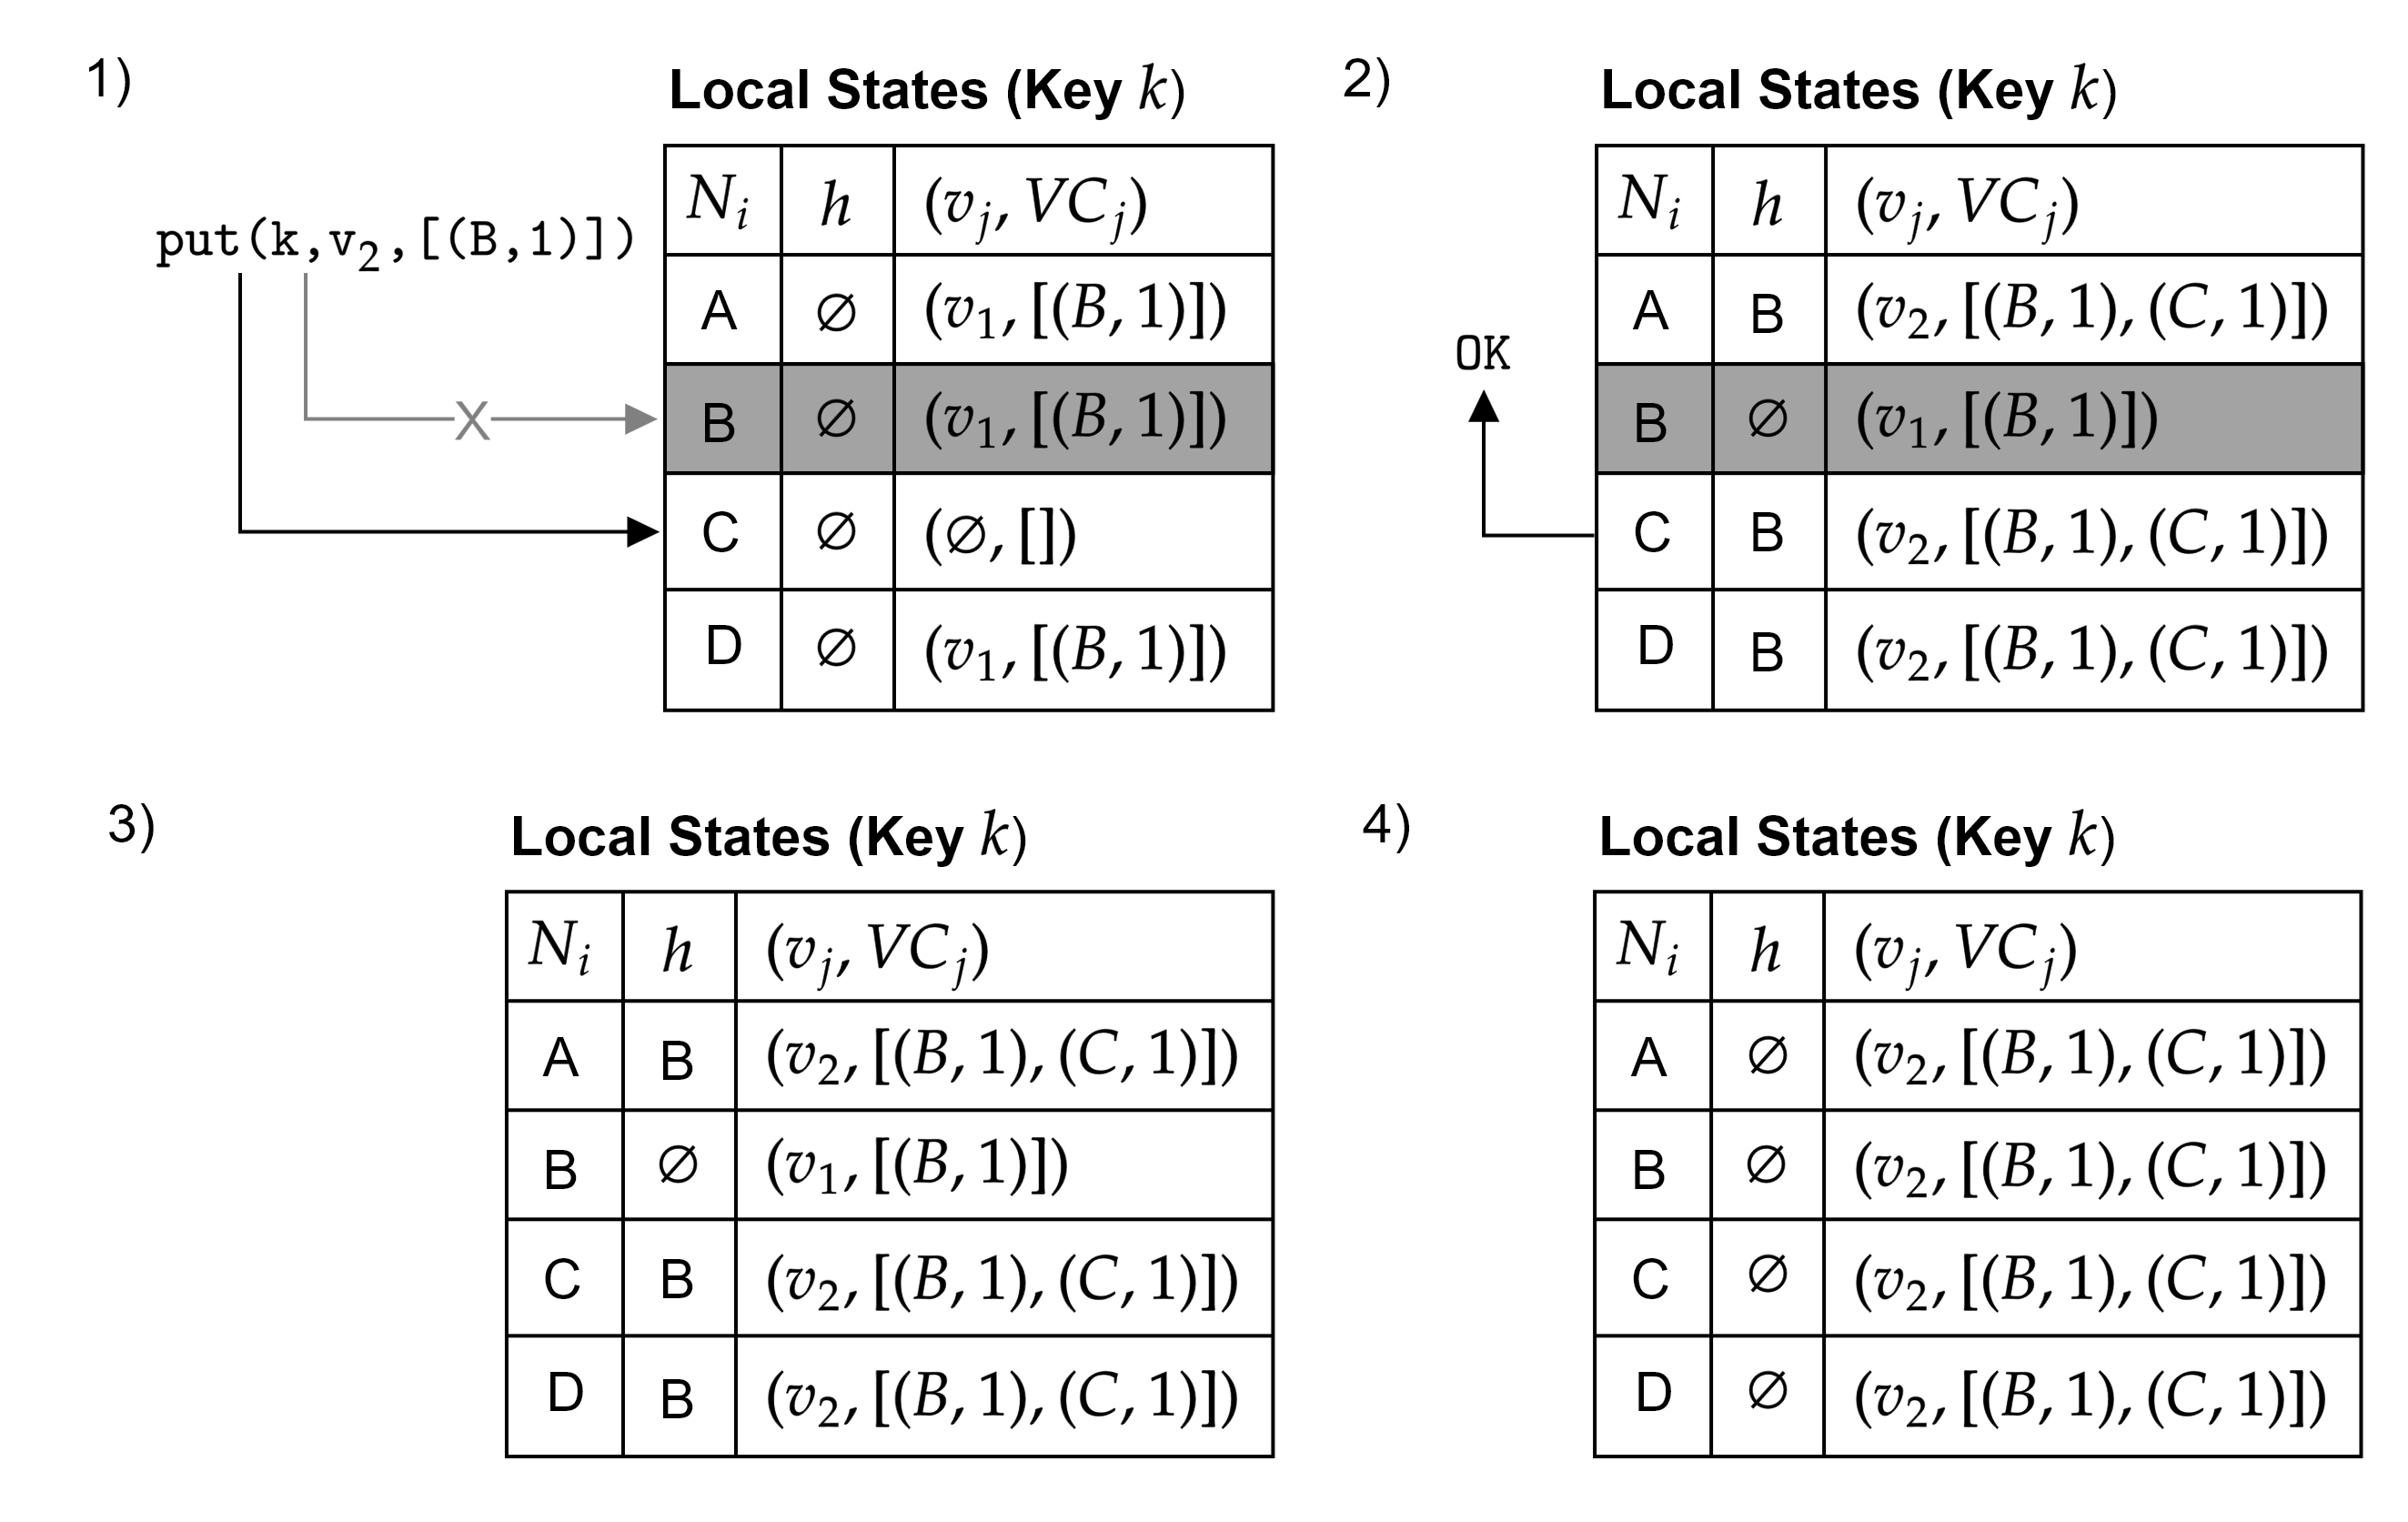
\includegraphics[width=\linewidth]{Sections/dyn/vc_2.png}\\
\noindent
\rule{\linewidth}{0.4pt}\\

\hspace{-1.5em}
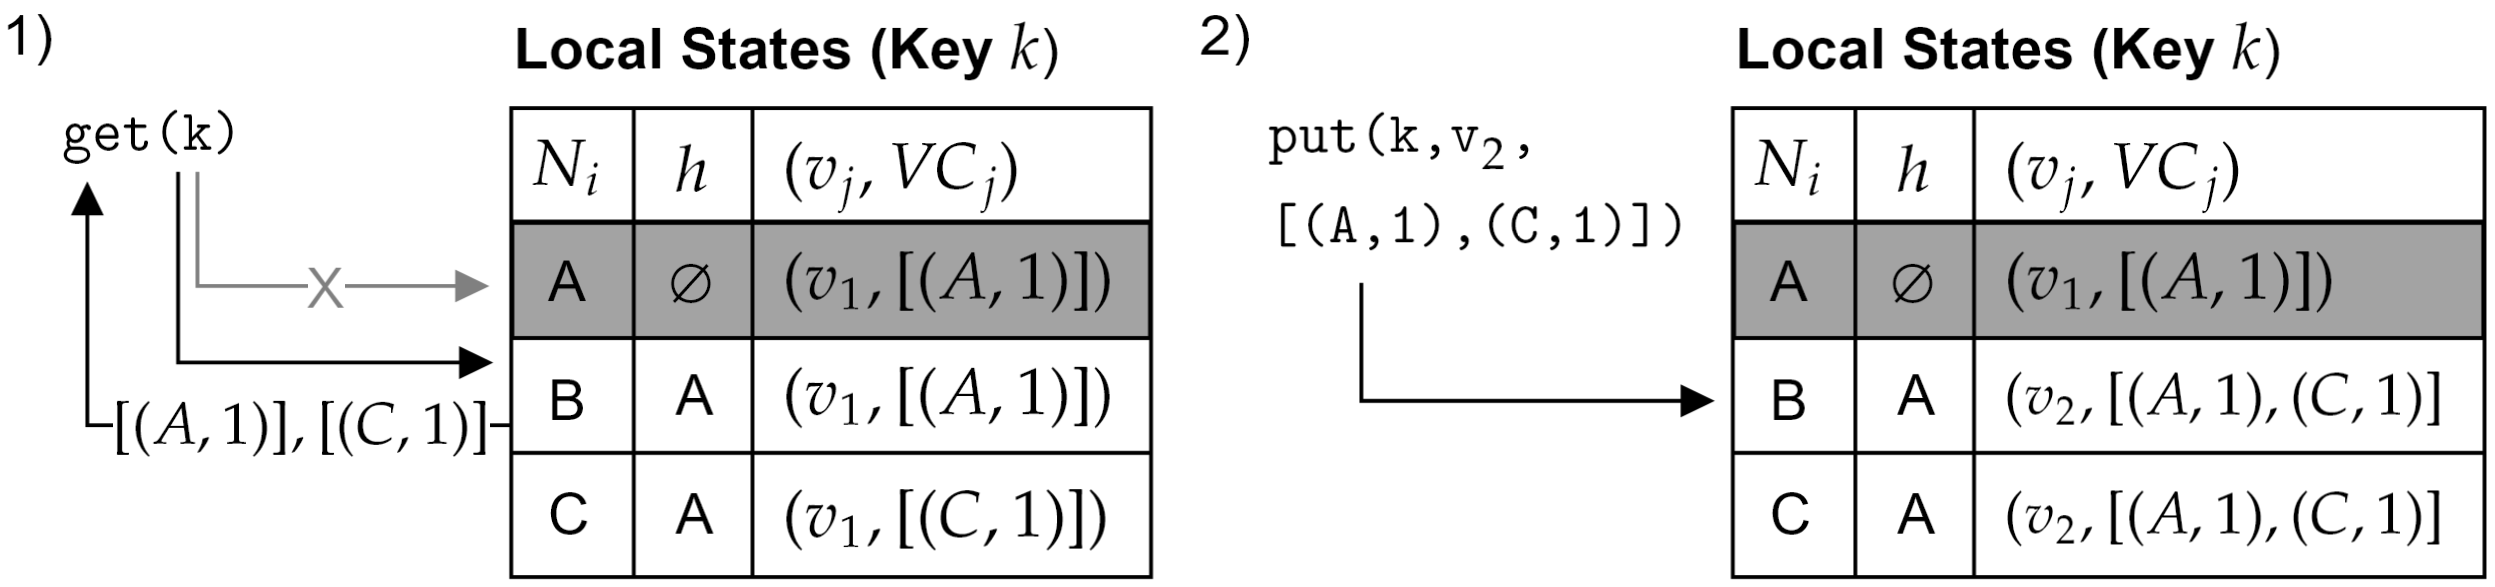
\includegraphics[width=\linewidth]{Sections/dyn/vc_3.png}\\

\vspace{.5em}
\noindent
\rule{\linewidth}{0.4pt}\\

\hspace{-1.5em}
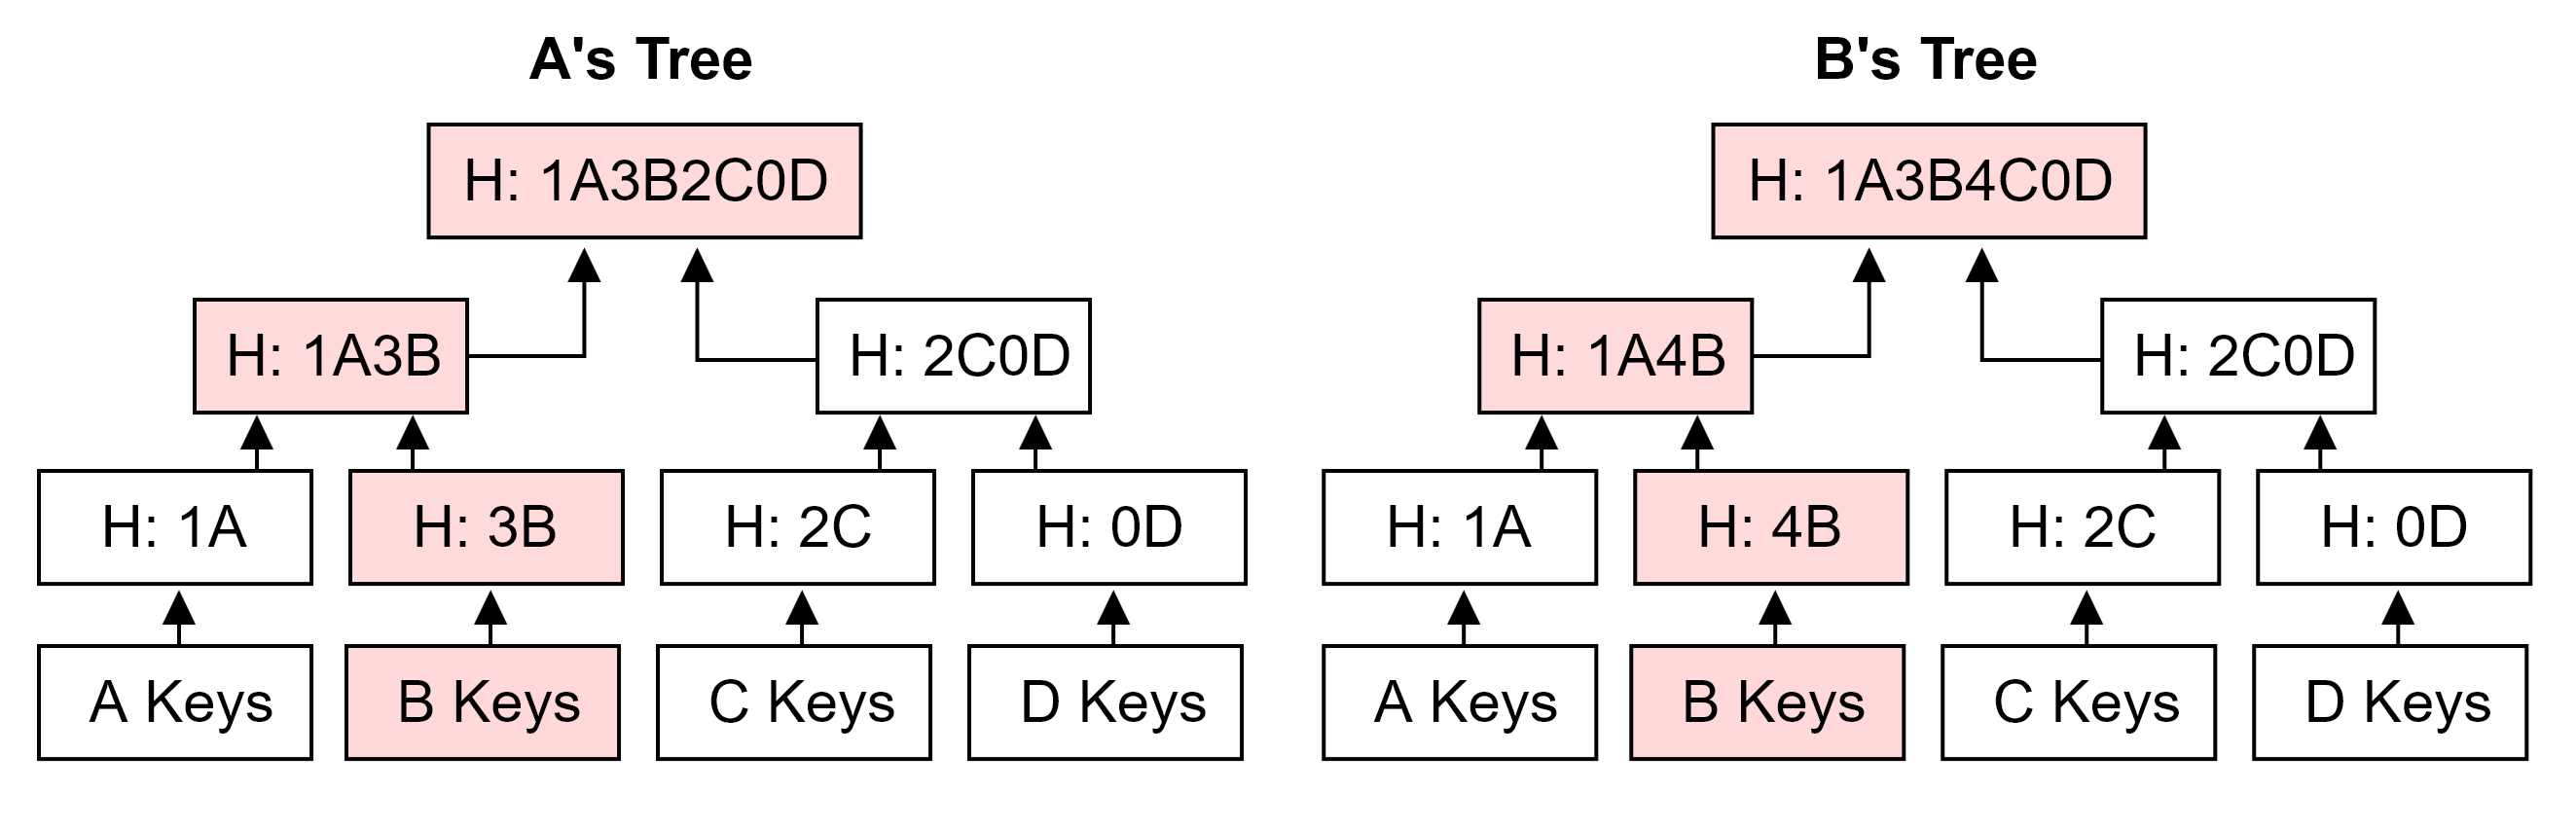
\includegraphics[width=\linewidth]{Sections/dyn/merkle.png}\\
\end{multicols}

\newpage

\noindent
$\delta$-time. 2PL2PC.



\begin{figure}[ht!]

    \centering
    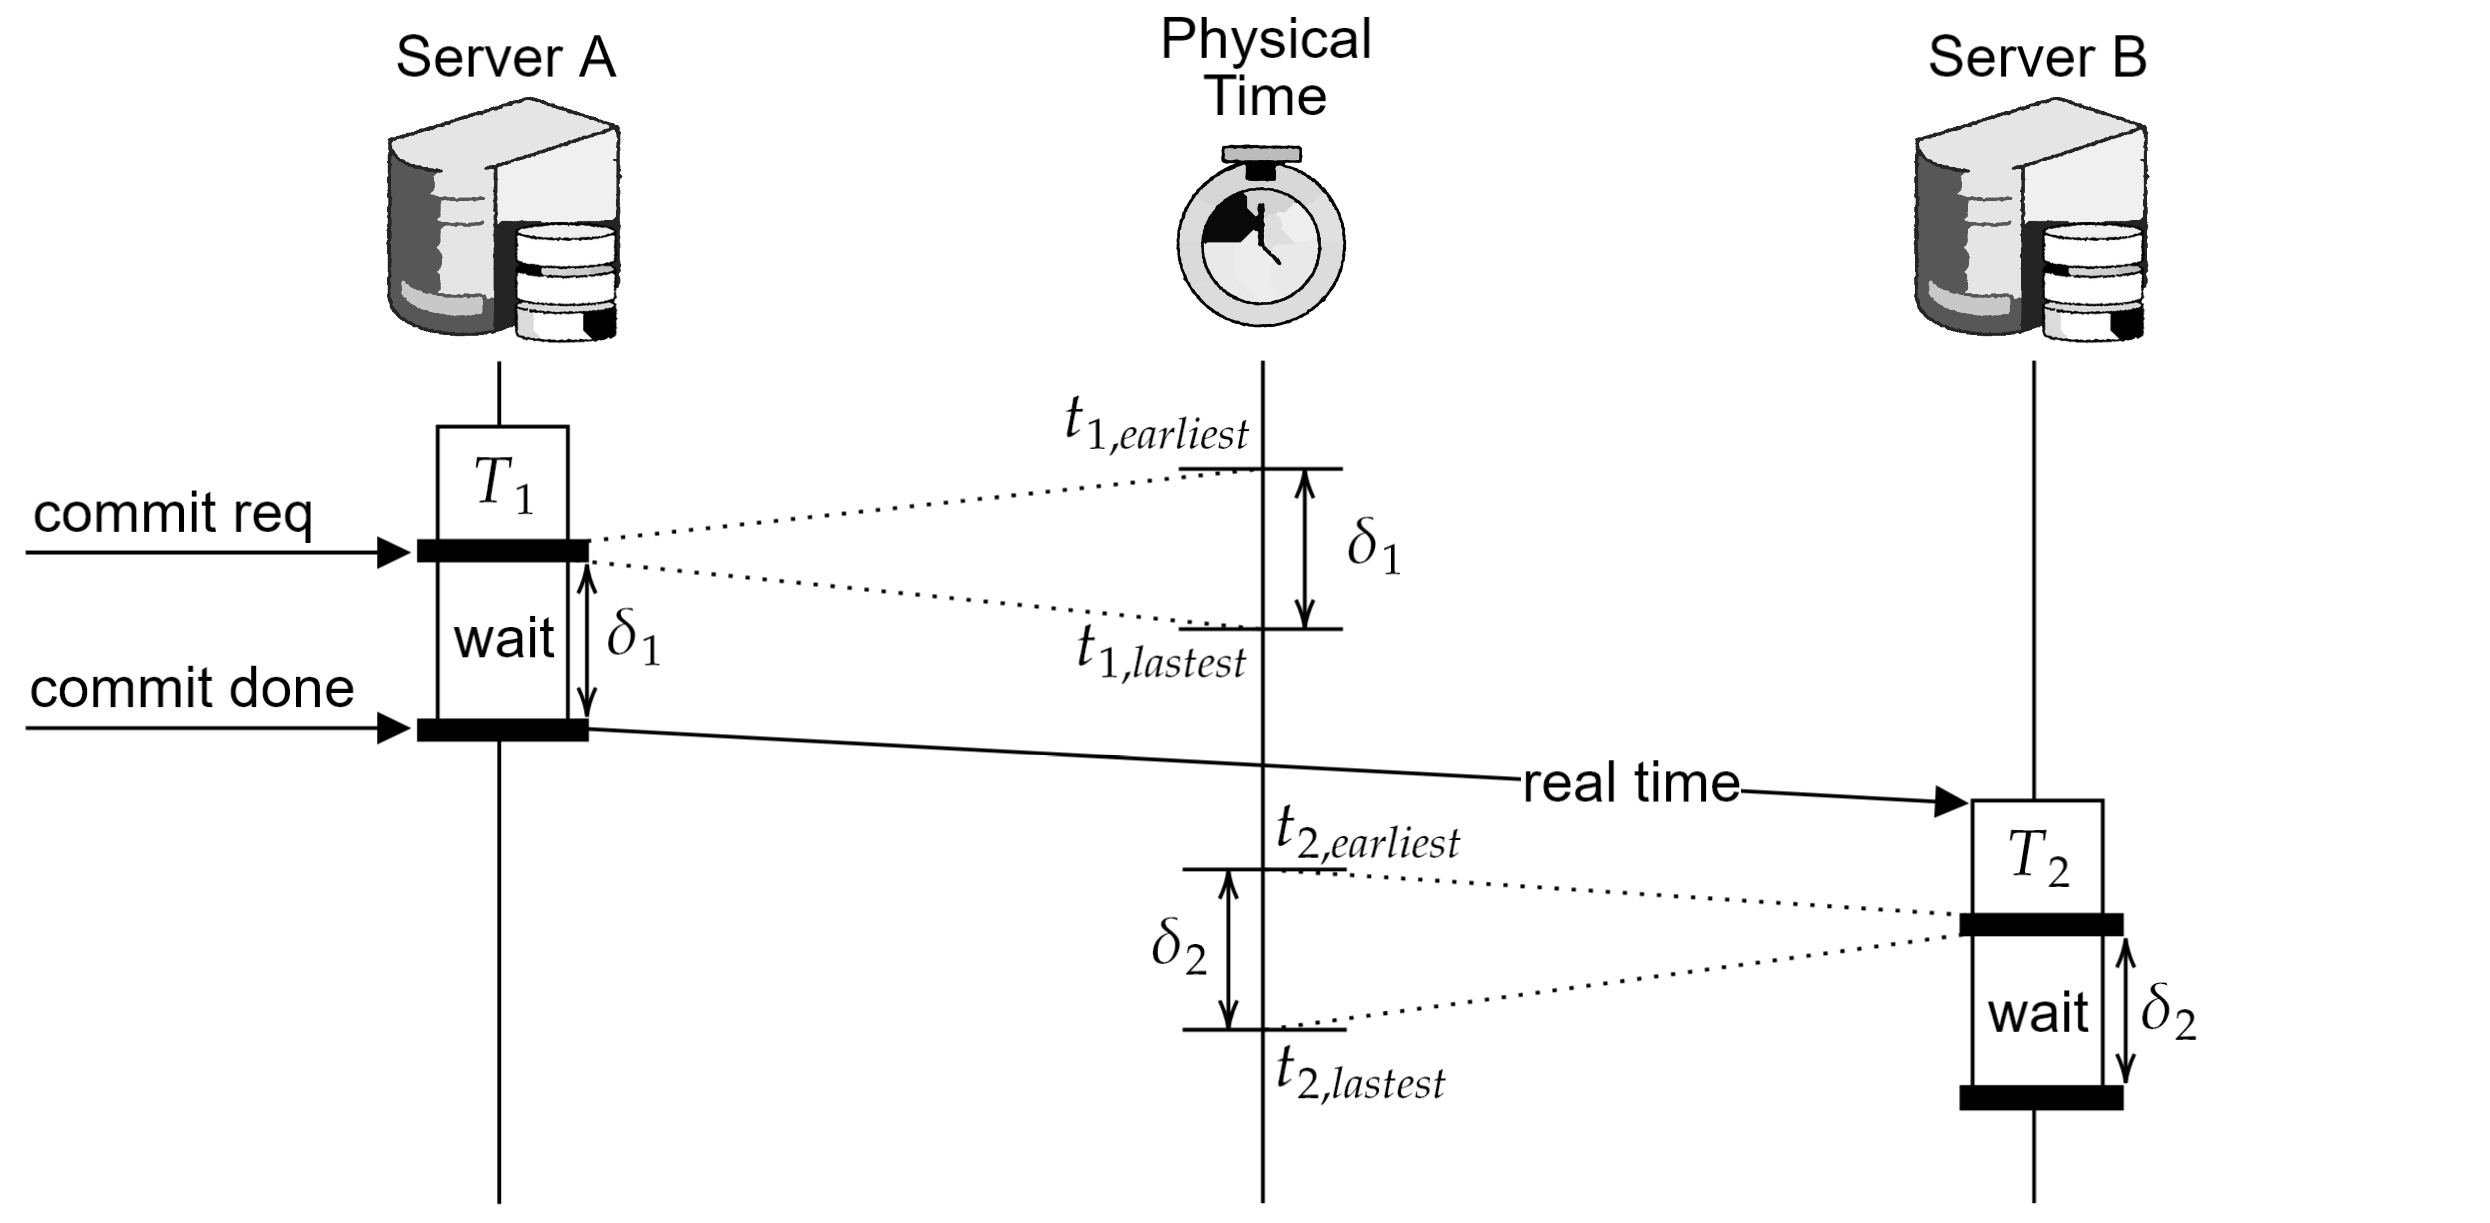
\includegraphics[width=\textwidth]{Sections/span/tt_2.png}
    \caption{Upon receiving a commit request, each coordinator (e.g.\ A) calls \texttt{TT.now()} and obtains an uncertainty interval \([t_{1,\mathrm{earliest}},\,t_{1,\mathrm{latest}}]\). It then delays for \(\delta_1 = t_{1,\mathrm{latest}} - t_{1,\mathrm{earliest}}\) before finalizing its commit timestamp.}
\end{figure}


\begin{figure}[ht!]
    \centering
    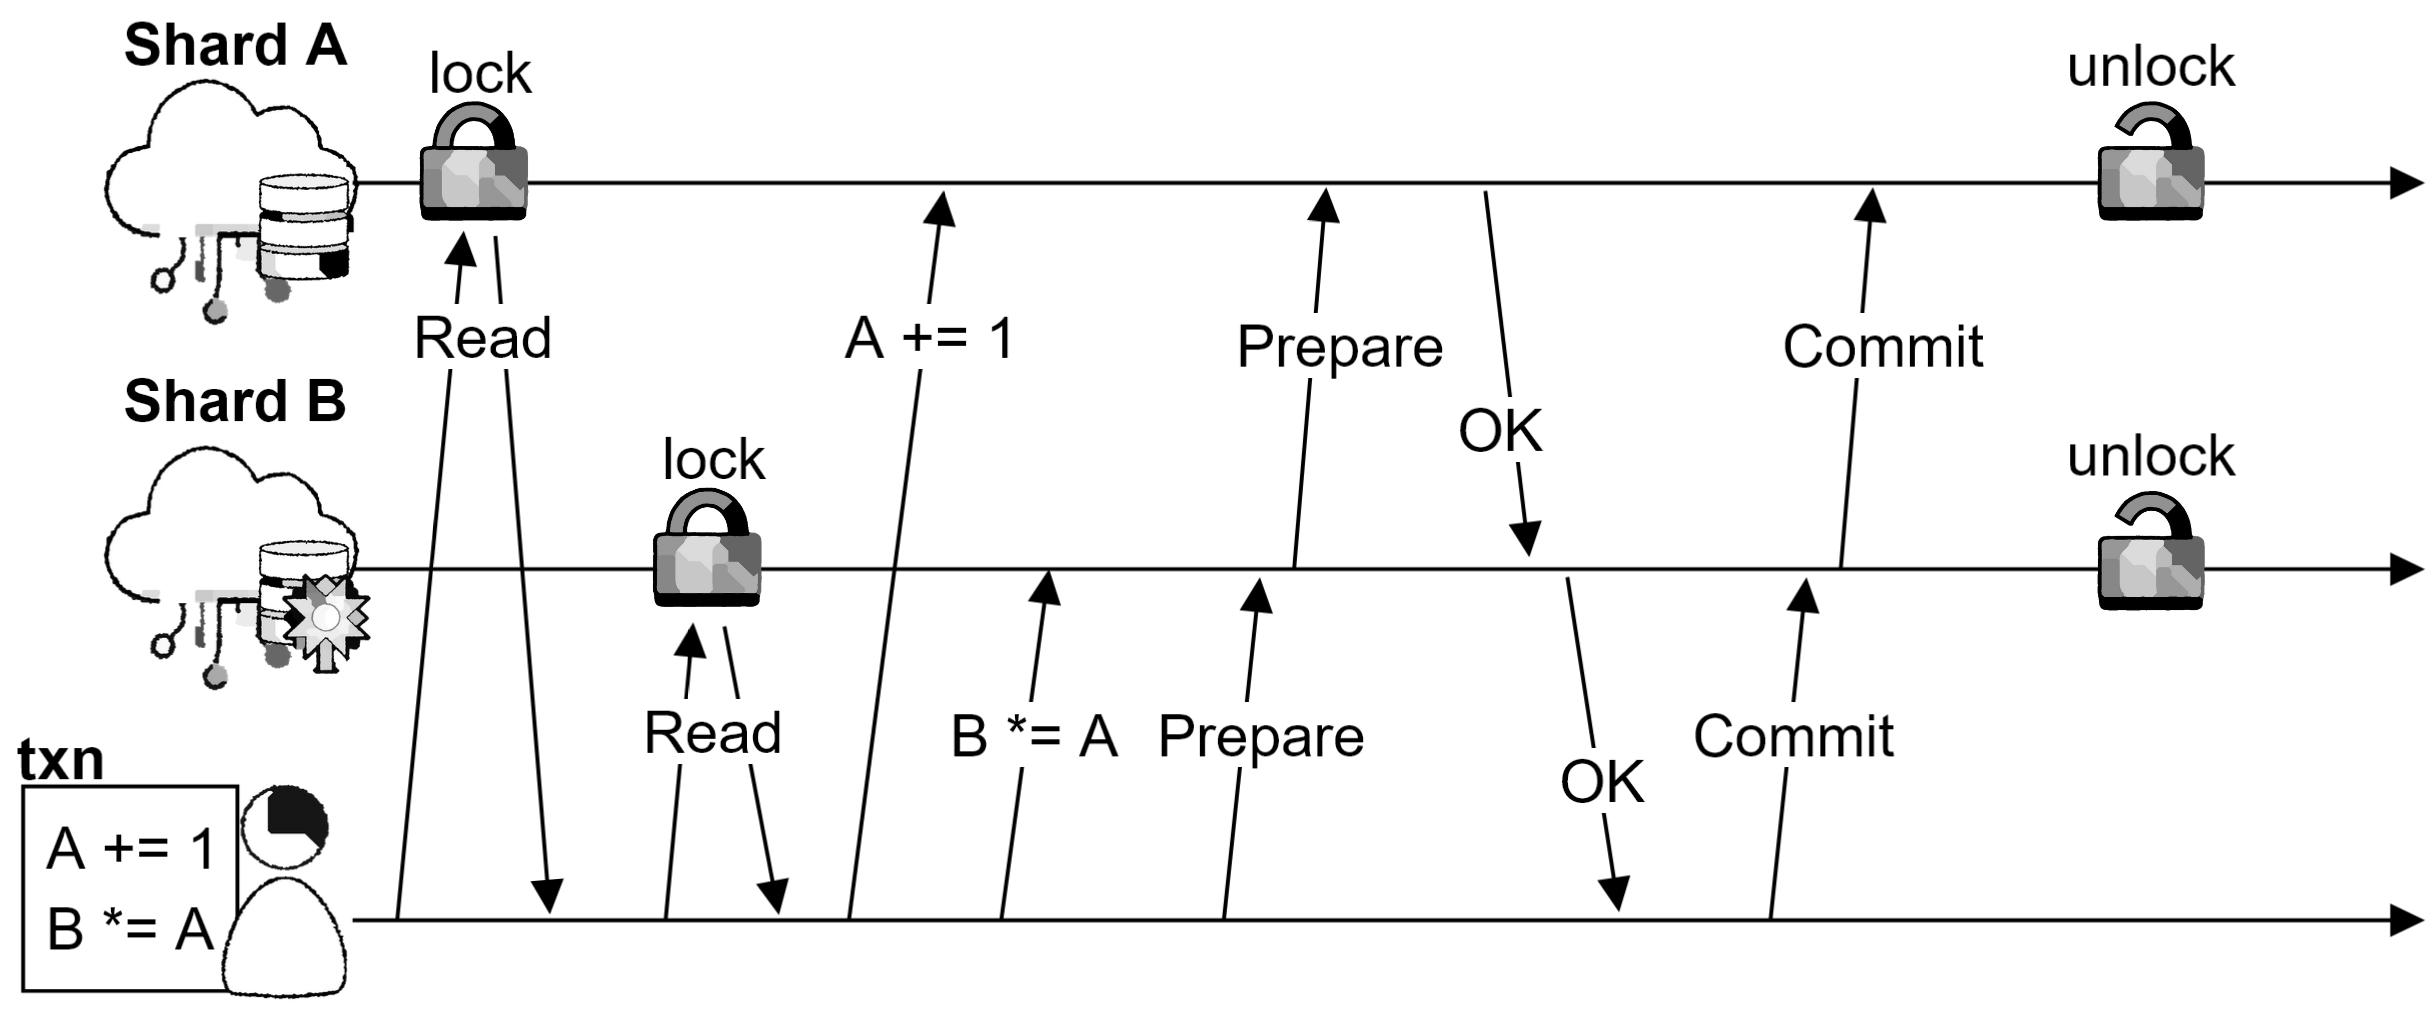
\includegraphics[width=\textwidth]{Sections/span/rw.png}
    \caption{A Read-Write Transaction 2PC Commit in Spanner, where txn is the transaction, $B$'s Paxos leader is the coordinator, and $A$ another participant. First, reads acquire locks, then 2PC begins.
    Commands are sent, and then the \texttt{PREPARE} and \texttt{COMMIT} phases begin, ending with the release of locks.}

\end{figure}

